
%\documentclass[12pt]{report}
%\documentclass[12pt]{extreport}
\documentclass[17pt]{extarticle}
%\documentclass{memoir}

\usepackage{graphicx}
\usepackage{setspace}
\usepackage{amsmath,amssymb}
\usepackage{IEEEtrantools}
\usepackage{cancel}
\usepackage[font=small,labelfont=bf]{caption}


\usepackage{verbatim}

\usepackage[T1]{fontenc}
\usepackage[utf8]{inputenc}
\usepackage[italian]{babel}


%\usepackage{imakeidx}%
%\makeindex[program=xindy]%, options=-C utf8 -L portuguese]%
\usepackage{makeidx}
\makeindex




\usepackage{geometry}
 \geometry{
 a4paper,
 total={170mm,264mm},
 left=20mm,
 top=10mm,
 }

\begin{document}

%\backmatter
%text\index{test}
\printindex

\begin{flushright}
{\bf \today}
\end{flushright}

\tableofcontents

\clearpage

La cinematica è quella branca della meccanica che studia il moto dei corpi indipendentemente dalle cause (le forze) che lo hanno determinato. La dinamica, invece, si occupa del moto dei corpi in relazione alle forze alle quali essi sono sottoposti.


\section{Richiami di moti rettilinei}

Le tre variabili principali della cinematica di un corpo sottoposto ad un moto rettilineo sono
\begin{itemize}
	\item posizione ($s$)
	\item velocità ($v$)
	\item accelerazione ($a$)
\end{itemize}

Il numero che identifica la distanza del corpo da un punto prescelto, detto origine, è la posizione $s$.

Quando il corpo è in moto, ossia la sua posizione varia nel tempo, allora il numero viene sostituito con una funzione della posizione rispetto al tempo 
\begin{eqnarray}
	\textbf{posizione}&\quad & s = s(t)
\end{eqnarray}

La velocità, a sua volta, è definita come la variazione della posizione rispetto al tempo(\emph{derivata prima}), mentre l'accelerazione è definita come la variazione della velocità rispetto al tempo (\emph{derivata prima}), o anche la derivata seconda della posizione rispetto al tempo

\begin{eqnarray}\label{eq:velocita}
	\textbf{velocità}& \qquad & v = \frac{\Delta s}{\Delta t}\\ \label{eq:accelerazione}
	\textbf{accelerazione}& \qquad & a = \frac{\Delta v}{\Delta t}
\end{eqnarray}

Espressioni pressochè equivalenti di velocità e accelerazione che si trovano su libri di testo di meccanica e, più in generale, di fisica, sono

\begin{eqnarray}
	\textbf{velocità}&\quad & v = \frac{ds}{dt}\\
	\textbf{accelerazione}&\quad & a = \frac{dv}{dt} = \frac{d^2s}{dt^2}
\end{eqnarray}

oppure ancora

\begin{eqnarray}
	\textbf{velocità}& \qquad & v = \dot{s}\\
	\textbf{accelerazione}& \qquad & a = \dot{v} = \ddot{s}
\end{eqnarray}


Nel sistema internazionale di unità di misura lo spostamento lo si esprime in metri ($m$), il tempo in secondi ($s$), la velocità in metri al secondo ($m/s$)\footnote{Il coefficente di conversione tra $m/s$ e $km/h$ è 3.6} e l'accelerazione in metri a secondo quadro ($m/s^2$).

Nei sottoparagrafi \ref{SPar:rettUn} e \ref{SPar:unAcc} ci sono due esempi in cui la posizione di un corpo viene espressa per mezzo di una funzione nel tempo $s(t)$.


\subsection{Moto rettilineo uniforme}\label{SPar:rettUn}

La cinematica di un corpo che si muove di moto rettilineo a velocità costante, sarà definito dalle equazioni

\begin{eqnarray}\label{eq:rettUniforme}
	v & = & \frac{\Delta s}{\Delta t} = \frac{s - s_0}{t - t_0}\\
	a & = & 0
\end{eqnarray}

La seconda di queste due equazioni deriva direttamente dalla definizione di velocità costante.
Dall'equazione \ref{eq:rettUniforme}, esplicitando $s$, e ponendo l'istante iniziale $t_0 = 0$, si ottiene la funzione $s(t)$
\begin{eqnarray}\label{eq:retUn}
	s & = & s_0 + vt
\end{eqnarray}

Ove ora $s$ è una funzione del tempo, $s_0$ è un parametro, noto come \emph{condizione iniziale}, nullo se il corpo si trova all'origine del sistema di riferimento al tempo $t = 0$. Il moto rettilineo uniforme può essere rappresentato da una retta in un grafico spazio-velocità (figura \ref{fig:graficoST_rettUniforme}).

\begin{figure}[h!]		
	\centering
   	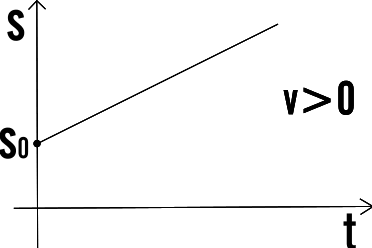
\includegraphics[width=1.8in]{graficoST_rettUniforme.png}
  	\caption{Grafico spazio-tempo del moto rettilineo uniforme}
   	\label{fig:graficoST_rettUniforme}
\end{figure}

Un esempio di applicazione della formula \ref{eq:retUn} è il seguente:\\
un auto viaggia a velocità costante $ v = 30m/s$ ($108km/h$), calcolare di quanto si sarà allontanata dopo 5 secondi
\begin{eqnarray}
	s = 0 + 30\cdot 5 = 150 m
\end{eqnarray}


\subsection{Moto rettilineo uniformemente accelerato}\label{SPar:unAcc}

Se il corpo non è a velocità costante, ma è sottoposto ad accelerazione $a$ costante, come potrebbe essere il caso di un grave in caduta libera, o un automobile in partenza da un semaforo, allora si dimostra che la cinematica del corpo può essere espressa dalle seguenti due equazioni\footnote{in un grafico velocità tempo, l'equazione della velocità \ref{eq:vel_accCost} è rappresentata da una retta, e lo spazio percorso è rappresentata dall'area di un triangolo \emph{sotto} la retta stessa.}

\begin{eqnarray}\label{eq:vel_accCost}
	v & = & v_0 + at\\ \label{eq:pos_accCost}
	s & = & s_0 + v_0t + \frac{1}{2}at^2
\end{eqnarray}


\begin{figure}[h!]		
	\centering
   	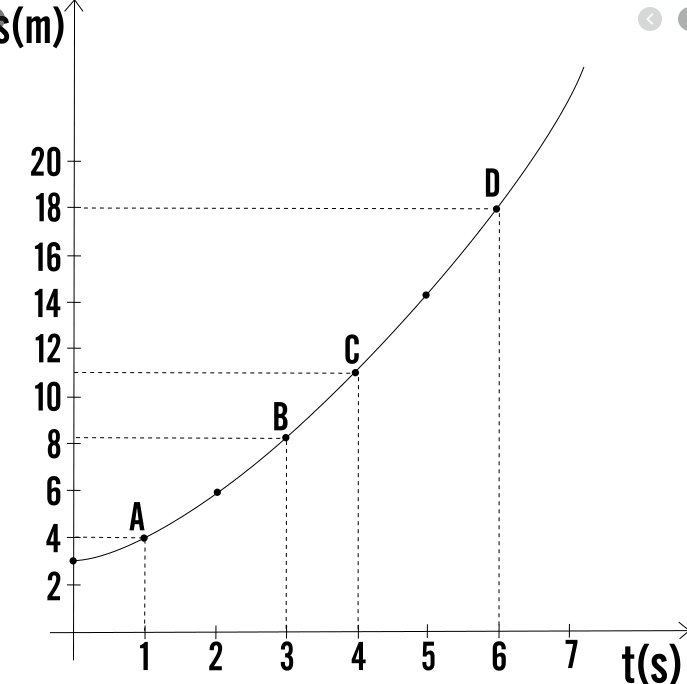
\includegraphics[width=1.8in]{graficoST_unAcc.png}%
  	\caption{Grafico spazio-tempo del moto uniformemente accelerato}
   	\label{fig:graficoST_unAcce}
\end{figure}

ove $s_0$ e $v_0$ sono, rispettivamente, la posizione e la velocità iniziale e sono nulle se il corpo parte da fermo da un punto coincidente con l'origine del sistema di riferimento. 

In un grafico s-t, il moto rettilineo uniformemente accelerato, espresso dall'equazione \ref{eq:pos_accCost}, viene rappresentato con una parabola (figura \ref{fig:graficoST_unAcce}).



Un esempio di applicazione delle equazioni \ref{eq:vel_accCost} e \ref{eq:pos_accCost} è quando si vuol conoscere la velocità e la posizione di un grave in caduta libera dopo un intervallo di tempo, ad esempio dopo 5 secondi. Sapendo che l'accelerazione di gravità è $a = 9.8m/s^2$ si ha
\begin{eqnarray}
	v & = & 9.8\cdot 5 = 49 m/s\\
	s & = & \frac{1}{2}9.8\cdot 5^2 = 122 m
\end{eqnarray}



\section{Richiami di Dinamica}
I tre principi della dinamica sono:

\begin{itemize}
	\item {\bf Primo Principio della Dinamica}
	Ogni corpo non sottoposto a forze si muove di moto rettilineo uniforme
	\item {\bf Secondo Principio della Dinamica (Legge di Newton)}
	Un corpo, dotato di massa $m$ e sottoposto ad una forza $\vec{F}$ è soggetto ad una accelerazione $\vec{a}$ pari a 
	
	\begin{eqnarray}\label{eq:Newton}
		\vec{F} = m \vec{a}
	\end{eqnarray}	
	Ove la forza si esprime in \emph{Newton} ($N$) e 1 $N$ è pari a 1 $kg\cdot m/s^2$.
	\item {\bf Terzo Principio della Dinamica}	
		se un oggetto A esercita una forza su un oggetto B, anche B esercita una forza su A. Le due forze sono uguali in intensità ma opposte in verso.
\end{itemize}


Dalla \ref{eq:Newton} si evince che se un corpo non è sottoposto a forze allora si muove di moto rettilineo uniforme (paragrafo \ref{SPar:rettUn}), se è sottoposto a una forza costante allora si muove di moto uniformemente accelerato (paragrafo \ref{SPar:unAcc}).


\subsection{Lavoro, energia e potenza}

In meccanica il lavoro di una forza $\vec{F}$ è il prodotto scalare della forza stessa per spostamento $\Delta \vec{s}$
\begin{eqnarray}\label{eq:Lavoro} 
	L = \vec{F}\cdot\Delta \vec{s}
\end{eqnarray}

Nel sistema internazionale il lavoro è spresso in \emph{Joule} (J).\\
Se forza e spostamento sono paralleli tra loro, allora l'equazione \ref{eq:Lavoro} si riduce a un semplice prodotto tra numeri.

\begin{eqnarray}\label{eq:LavoroS}
	L = F\Delta s
\end{eqnarray}

Il lavoro necessario per portare un corpo di massa $m$ a una velocità $v$ è noto come \emph{energia cinetica} $K$ ed è espresso dalla seguente formula%\footnote{In un grafico lavoro-spostamento, l'equazione \ref{eq:LavoroS} è rappresentata da una retta passante per l'origne, e l'energia cinetica è rappresentata dall'area di un triangolo che sta sotto la retta }

\begin{eqnarray}
	K = \frac{1}{2}mv^2
\end{eqnarray}

Ci sono grandezze fisiche per le quali il lavoro compiuto \emph{non} dipende dal particolare percorso svolto, ma dipende \emph{soltanto} dal punto di partenza e il punto finale. Queste forze si chiamano \emph{conservative}. Per queste forze possiamo definire una \emph{energia potenziale} $U$ 

\begin{eqnarray}\label{eq:Potenziale}
	L_c = -\Delta U = U_i -U_f
\end{eqnarray}

Esempi di forze conservative sono
\begin{itemize}
	\item forza gravitazionale
	\item forza elettrica
	\item forza elastica (oscillatore armonico)
\end{itemize}

In realtà un corpo in moto è \emph{sempre} sottoposto, non soltanto a forze conservative, ma anche a forze non conservative. La forza non conservativa più importante è la forza d'attrito, e dissipa l'energia sotto forma di calore. In generale, il lavoro totale speso per spostare un corpo da un punto inziale ad un punto finale è la somma del lavoro delle forze conservative $L_c$ (come la forza elettrica) e di quelle non conservative $L_{nc}$ (come la forza d'attrito)

\begin{eqnarray}
	L = L_{c} + L_{nc}
\end{eqnarray}

Si dimostra, inoltre, che in un moto da un punto iniziale ad un punto finale, il lavoro di una forza agente sul corpo è dato dalla differenza di energia cinetica 
\begin{eqnarray}\label{eq:Cinetica}
	L = \Delta K
\end{eqnarray}

Dalle equazioni \ref{eq:Potenziale} e \ref{eq:Cinetica} si dimostra il teorema di conservazione dell'energia
\begin{eqnarray}\label{eq:Energia}
	K_i + U_i = K_f + U_f + L_{nc}
\end{eqnarray}


Il lavoro delle forze non conservative $L_{nc}$, in particolar modo il lavoro delle forze d'attrito viene dissipato sotto forma di calore. 

L'equazione \ref{eq:Energia} esprime che l'energia non si crea e non si distrugge ma, durante un qualsiasi processo, si trasforma in forme diverse. Secondo l'equazione \ref{eq:Energia}, un corpo, dopo che è stato sottoposto ad uno spostamento per effetto di una forza, sarà dotato di una energia \emph{minore} perchè parte di quella energia sarà andata dispersa sotto forma di calore per effetto di forze non conservative (l'attrito!) il cui lavoro è dato dal termine $L_{nc}$.

Si definisce \emph{potenza} la quantità di lavoro speso nell'unità di tempo

\begin{eqnarray}\label{eq:Potenza}
	P = \frac{L}{\Delta t}
\end{eqnarray}

Se l'intervallo di tempo è il secondo, allora la potenza si sprime in Watt. Dall'equazione \ref{eq:LavoroS} e l'equazione \ref{eq:Potenza} si evince che la potenza di un corpo in moto è data dal prodotto forza per velocità\footnote{Come l'equazione del lavoro \ref{eq:LavoroS} è una semplificazione di un caso più generale, che tiene conto di complicazioni di carattere geometrico, così l'equazione \ref{eq:Potenza1} è una semplificazione di una equazione più generale, che tiene conto di complicazioni di carattere geometrico, e che è $P=\vec{F}\cdot\vec{v}$. }

\begin{eqnarray}\label{eq:Potenza1}
	P = \frac{F\Delta s}{\Delta t} = Fv
\end{eqnarray}




\section{Moto circolare}



Esaminiamo ora il moto di un corpo che si muove lungo una circonferenza quale, ad esempio, un corpo che si trova vincolato al rotore di un motore elettrico.  

Prima di procedere è bene fare un ripasso del concetto di angolo in radianti.\\
L'espressione dell'angolo in radianti è, per sua stessa definizione, il rapporto tra l'arco di circonferenza $\Delta s$ e il raggio (figura \ref{fig:arcoCirconferenza})

\begin{eqnarray}\label{eq:angolo}
	\alpha = \frac{\Delta s}{r}
\end{eqnarray}






\begin{figure}[h!]		
	\centering
   	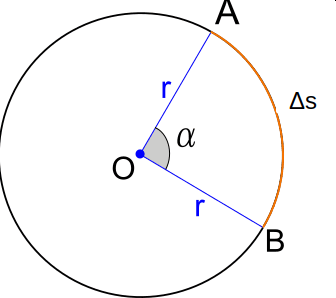
\includegraphics[width=1.8in]{arcoCirconferenza.png}%graficoST_rettUniforme.png
  	\caption{Espressione in radianti dell'arco di circonferenza.}
   	\label{fig:arcoCirconferenza}
\end{figure}


Infatti il valore $2\pi$ associato ad un angolo giro deriva dall'equazione del perimentro della circonferenza ($p = 2\pi r$) e l'equazione \ref{eq:angolo} 



\begin{eqnarray}
	\textbf{angolo giro in radianti}\qquad \alpha = \frac{2\pi r}{r} = 2\pi
\end{eqnarray}


\subsection{Cinematica del moto circolare}
Anche nei moti circolari si possono usare le equazioni \ref{eq:velocita} e \ref{eq:accelerazione}, ove la variazione di spazio ora coincide con l'arco di circonferenza spazzato dal punto materiale nell'unità di tempo. In questi casi la velocità e l'accelerazione si chiamano, rispettivamente, \emph{velocità tangenziale} e \emph{accelerazione tangenziale}.


Tuttavia, in perfetta analogia con quanto fatto per i moti rettilinei, con l'angolo $\alpha$ definiamo la posizione del punto materiale, mentre con la derivata dell'angolo $\alpha$ rispetto al tempo definiamo la velocità angolare $\omega$ e con la derivata della velocità angolare rispetto al tempo definiamo l'accelerazione angolare

\begin{eqnarray}
	\textbf{velocità angolare} &\qquad & \omega = \frac{d\alpha}{dt}\\
	\textbf{accelerazione angolare} &\qquad & \dot{\omega} = \frac{d \omega}{dt}
\end{eqnarray}


Si ricava, quindi, che la relazione sussistente tra velocità posizione e angolo, la relazione sussistente tra velocità tangenziale e velocità angolare, nonchè la relazione sussistente tra accelerazione tangenziale e accelerazione angolare è

\begin{eqnarray}
	s = r\alpha \\ \label{eq:velAng}
	v = r\omega \\ \label{eq:accAng}
	a = r\dot{\omega}
\end{eqnarray} 






\subsection{Dinamica del moto circolare di un corpo estesso}\label{cap:corpoRigido}

Affinchè un corpo esteso (corpo rigido) sia sottoposto ad una rotazione, è necessario che sia presente una \emph{coppia di forze}, uguali in intensità e in direzione opposta e applicate in due punti distinti del corpo stesso (figura \ref{fig:Coppia}). 

Pontendoci in una configurazione geometrica elementare, come quella di figura \ref{fig:Coppia}, si definisce coppia $C_m$ il prodotto dell'intensità della forza per la distanza $d = 2r$ rispetto ai due punti di applicazione

\begin{eqnarray}
	C_m = 2rF
\end{eqnarray}

L'unità di misura della coppia nel sistema internazionale è Newton per metro ($Nm$).

%Una tale configurazione si 
%Sotto una tale configurazione il corpo sarà sottoposto ad una rotazione intorno al punto intermedio (figura \ref{fig:Coppia}). 



\begin{figure}[ht!]		
	\centering
   	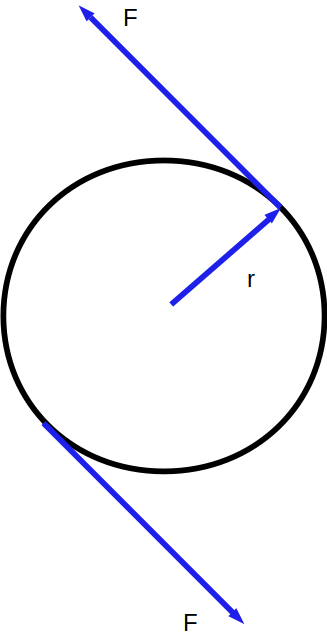
\includegraphics[width=1.6in]{Coppia.png}%graficoST_rettUniforme.png
  	\caption{Una rotazione di un corpo rigido la si ottiene se e solo se è presente una \emph{coppia}}
   	\label{fig:Coppia}
\end{figure}

Si può ottenere una tale configurazione applicando una singola forza ad un corpo vincolato a ruotare attorno a un asse fisso, come quando si gira con una mano la ruota di una bicicletta\footnote{La reazione vincolare dell'asse della ruota costituisce la seconda forza della "coppia".}, oppure applicando due distinte forze in due punti distinti, in modo tale che l'asse di rotazione sia passante per il punto intermedio rispetto ai due punti di applicazione della forza, come accade sul rotore del motore elettrico.


\'E evidente che l'effetto di una forza, ai fini di una rotazione, non dipende soltanto dalla sua intensità, ma dipende anche dalla distanza del punto di applicazione di questa forza rispetto all'asse di rotazione. 

Ponendoci, per semplicità, in una configurazione geometrica più semplice possibile, come quella in figura \ref{fig:Coppia}, per studiare i moti rotativi, si usa non soltanto la forza, ma il prodotto della forza $F$ per la distanza $r$ rispetto all'asse di rotazione. 


\begin{eqnarray}
	M = rF
\end{eqnarray}

dove $M$ è il \emph{momento della forza} e $r$ è il \emph{braccio} della forza.



Moltiplicando a destra e a sinistra, l'equazione di Newton (equazione \ref{eq:Newton}) per il raggio $r$ si ha
\begin{eqnarray}\label{eq:Momento}
	M = rF = mar
\end{eqnarray}

usando l'espressione dell'equazione \ref{eq:accAng}, nell'equazione \ref{eq:Momento}, e sostituendo $I = mr^2$ si ha

\begin{eqnarray}\label{Momento1}
	M = I\dot{\omega}
\end{eqnarray}

Ove


\begin{itemize}
	\item $M$ è il momento della forza
	\item $I = mr^2$ si chiama \emph{momento d'inerzia}
	\item $\dot{\omega}$ è l'accelerazione angolare
\end{itemize}


Nella presente trattazione abbia considerato una gemetria elementare del corpo rigido e delle forze applicate su di esso. In generale si presentano due complicazioni: 

\begin{itemize}
	\item le forze non sono necessariamente perpendicolari alla circonferenza, come invece accade in figura \ref{fig:Coppia}. Per sopperire a queste complicazioni di carattere geometrico, il momento di una forza viene definito dal prodotto vettoriale
		\begin{eqnarray}
			\vec{M} = \vec{r}\times\vec{F} 	
		\end{eqnarray}
		
	Evidentemente anche l'accelerazione angolare $\dot{\omega}$ diventa un vettore, tra l'altro parallelo a $\vec{M}$, e l'equazione \ref{Momento1} diventa
	
		\begin{eqnarray}
			\vec{M} = I \vec{\dot{\omega}}
		\end{eqnarray}
	\item le differenti parti del corpo rigido, non sono disposte lungo una figura geometrica ad anello, ma si trovano a differente distanza rispetto all'asse di rotazione. Esempi di questo genere possono essere, ad esempio, una sfera che gira intorno a se stessa o un cilindro che gira intorno al suo asse di rotazione, oppure il rotore di un motore elettrico che sicuramente non avrà una forma ad anello. In tali casi occorre generalizzare il concetto di momento d'inerzia, facendo uso di un integrale

\begin{eqnarray}\label{eq:momInerzia}
	I = \int r^2dm
\end{eqnarray}	
	
\end{itemize}






\begin{figure}[b!]		
	\centering
   	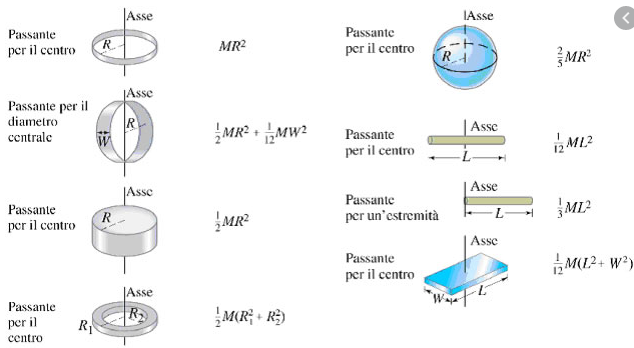
\includegraphics[width=4.3in]{momentiDInerzia.png}%arcoCirconferenza.jpg
  	\caption{Tabella di momenti d'inerzia di differenti figure geometriche, calcolate facendo uso dell'equazione \ref{eq:momInerzia}.}
   	\label{fig:momentiDInerzia}%ForzaLorentz.png
\end{figure}


Proseguendo in questa direzione, benchè la trattazione si fa velocemente assai complessa dal punto di vista matematico, tuttavia l'equazione dei momenti \ref{eq:Momento} e l'equazione di Newton \ref{eq:Newton} hanno la stessa identica forma matematica. E quindi, come l'assenza di forze generi un moto rettilineo uniforme (paragrafo \ref{SPar:rettUn}), così l'assenza di momenti genera un moto circolare uniforme, descritto dalle equazioni

\begin{eqnarray}
	\alpha & = & \alpha_0 + \omega t\\
	\dot{\omega} & = & 0
\end{eqnarray}

Allo stesso modo, come l'applicazione di una forza costante genera un moto rettilineo uniformemente accelerato (paragrafo \ref{SPar:unAcc}), così l'applicazione di un momento genera un moto circolare uniformemente accelerato, descritto dalle equazioni

\begin{eqnarray}
	\alpha & = & \alpha_0 + \omega_0 t + \frac{1}{2}\dot{\omega}t^2\\
	\omega & = & \omega_0 + \dot{\omega}t
\end{eqnarray}


\begin{figure}[ht!]		
	\centering
   	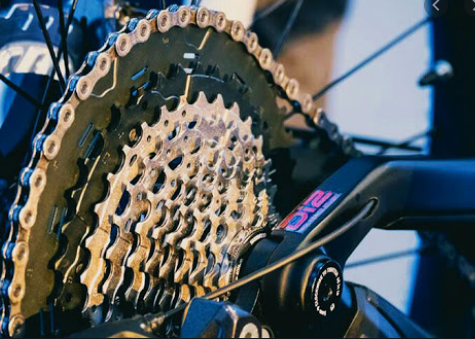
\includegraphics[width=2.8in]{coppiaAlta.png}
   	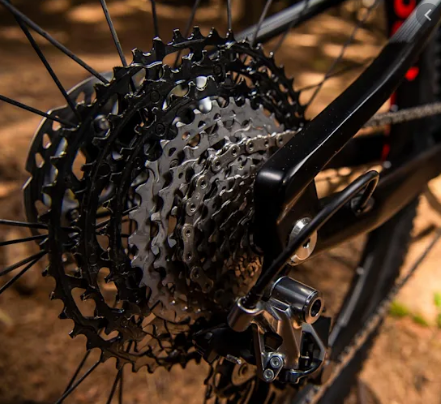
\includegraphics[width=2.2in]{coppiaBassa.png}
  	\caption{A parità di potenza (equazione \ref{eq:PotenzaR}) a sinistra il sistema meccanico è dotato di una coppia alta e una velocità angolare bassa. Mentre a destra è dotato di una coppia bassa e una velocità angolare alta.}
   	\label{fig:coppiaBassaAlta}
\end{figure}


Allo stesso modo, come il lavoro di un corpo su moto rettilineo è il prodotto di forza per spostamento (equazione \ref{eq:LavoroS}), così il lavoro di un forza su un corpo rigido in rotazione può essere espresso dal prodotto del momento per l'angolo

\begin{eqnarray}
	L = M\alpha
\end{eqnarray}

Infine, la potenza, che è definita come lavoro per unità di tempo (equazione \ref{eq:Potenza}), nei moti rettilinei è pari a forza per velocità (equazione \ref{eq:Potenza1}), nei moti rotatori è momento per velocità angolare\footnote{Anche qui, per assolvere a problematiche che si presentano in casi di dinamiche e geometrie più complicate, come ad esempio il moto di rotazione di una trottola non soltanto attorno al suo asse di rotazione, ma anche il moto di rotazione dell'asse stesso (precessione), l'equazione \ref{eq:PotenzaR} assume una forma vettoriale del tipo $\vec{P} = M\vec{\omega}$. }

\begin{eqnarray}\label{eq:PotenzaR}
	P = M\omega
\end{eqnarray} 


Per capire il significato dell'equazione \ref{eq:PotenzaR} consideriamo il moto di un ciclista su una bicicletta con le marce. Supponiamo che la potenza massima $P$ che il ciclista riesce ead esprimere sia di $400$ $Watt$. Con tale potenza il ciclista può richiedere una \emph{alta coppia} (figura \ref{fig:coppiaBassaAlta}, lato sinistro), e quindi riuscire a trasportare un carico impegnativo a discapito però della velocità. Oppure può ridurre la coppia (figura \ref{fig:coppiaBassaAlta}, lato destro), e quindi ridurre il carico trasportabile, ma guadagnando in velocità.


\clearpage








\section{Il Campo magnetico}


La presente lezione si propone di spiegare, per somme linee, cos'è il campo magnetico e alcune delle sue più importanti applicazioni quali l'induttanza e il trasformatore. 


\begin{figure}[b!]		
	\centering
   	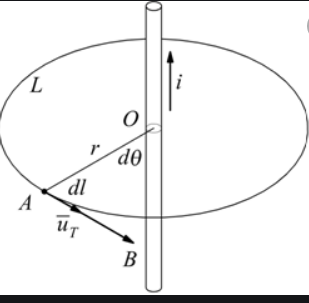
\includegraphics[width=2.8in]{FiloRettilineoCorrente_B.jpg}		%rettaNONpassOrig.jpg
  	\caption{Campo magnetico $\vec{B}$ generato da un filo rettilineo percorso da corrente $i$. La linea circolare in prospettiva rappresenta una linea (chiusa) di campo magnetico.}
   	\label{fig:FiloRettilineoCorrente_B}
\end{figure}




Data una corrente elettrica, intorno ad essa si genera un campo vettoriale che prende il nome di campo magnetico, tipicamente rappresentato matematicamente con la variabile $\vec{B}$, e rappresentato graficamente per mezzo di \emph{linee di campo chiuse}\footnote{Si dice che il campo magnetico, essendo rappresentabile da linee di campo chiuse, è \emph{irrotazionale} }(figura \ref{fig:FiloRettilineoCorrente_B}). 

\emph{Ciascun punto della linea di campo rappresenta la direzione del campo magnetico nel punto stesso}. Il verso del vettore campo magnetico va dal cosiddetto \emph{polo nord} al cosiddetto \emph{polo sud}.
Un campo magnetico può essere generato anche da correnti permanentemente presenti all'interno di alcuni materiali speciali, detti \emph{magneti}. Oppure può essere \emph{acceso} da correnti esterne in materiali detti \emph{ferromagneti}.

La natura del campo magnetico (modulo, direzione, verso e dipendenza dalla posizione) dipende, chiaramente, dalla geometria del percorso 
della corrente che lo induce e, di conseguenza, può presentare una notevole complessità matematica.





\begin{figure}[b!]		
	\centering
   	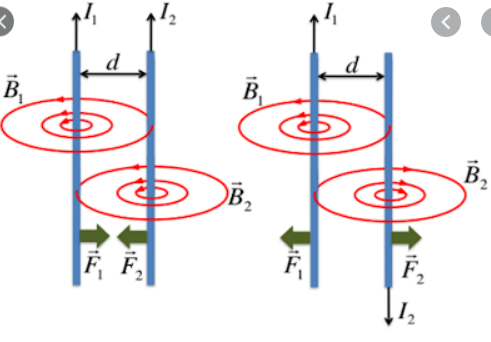
\includegraphics[width=2.8in]{campoMagneticoFiliParalleli.png}	
  	\caption{Forza di interazione magnetica (frecce verdi) tra due fili paralleli percorsi da corrente (linee blu verticali). Linee di campo magnetio $\vec{B}$ generate da ciascun filo percorso da corrente}
   	\label{fig:campoMagneticoFiliParalleli}%ForzaLorentz.png
\end{figure}






Le due principali unità di misura del campo magnetico sono il \emph{Tesla} (Sistema internazionale) ed il \emph{Gauss}. $1 Tesla = 10^4 Gauss$.














\subsection{Effetti del campo magnetico }


%L'orientazione reciproca delle correnti
%La differenza tra "polo sud magnetico" e "polo nord magnetico" \'e data, appunto, dal fatto che, a seconda dell'orientazione 

%Come \'e ben noto, esistono materiali speciali, detti magneti, i quali sono in grado di generare un campo magnetico intorno a se. Ci\'o \'e dovuto al fatto che in questi materiali ci sono degli elettroni che generano delle correnti elettriche interne sufficientemente intense da provocare fenomeni di attrazione/repulsione con altri magneti o con metalli.




Essenzialmente la presenza di un campo magnetico può dar luogo a due effetti: una forza (\emph{Forza di Lorentz}) o una tensione indotta (\emph{Legge di Faraday Neumann}).
\begin{enumerate}
	\item 
	{\bf Forza di Lorentz}
	
	
Una forza (si esprime in Newton) sulle cariche di una corrente elettrica, perpendicolare sia alla direzione del campo magnetico $\vec{B}$ che alla direzione della corrente $\vec{l}$ e responsabile dell'\emph{Effetto Hall} (figura \ref{fig:EffettoHall}), fenomeno di largo impiego nella trasduzione.


Tale forza è data dall'\emph{Equazione di Lorentz} (figura \ref{fig:ForzaLorentz} )
	
 	
\begin{eqnarray}\label{eq:Lorentz}
	 \vec{F} = i\vec{l}\times\vec{B}
\end{eqnarray}	
	
(prodotto vettoriale)\footnote{Una analoga formulazione della Legge di Lorentz è $\vec{F}= q\vec{v}\times \vec{B}$, ove $q$ è la carica dell'elettrone e $v$ è la velocità. il prodotto $q\vec{v}$ è identico al prodotto $i\vec{l}$. }. 

Il verso può essere ricavato facendo uso della regola della mano destra (figura \ref{fig:manoDestra}) .

In pratica, sarà di attrazione o di repulsione a seconda dell'orientazione reciproca della corrente che genera il campo magnetico e la corrente che da tale campo magnetico viene investito \footnote{Questa forza è, nella maggior parte dei casi, molto piccola e quindi trascurabile. } (figura \ref{fig:campoMagneticoFiliParalleli}). 


\begin{figure}[bh!]
	\centering
   	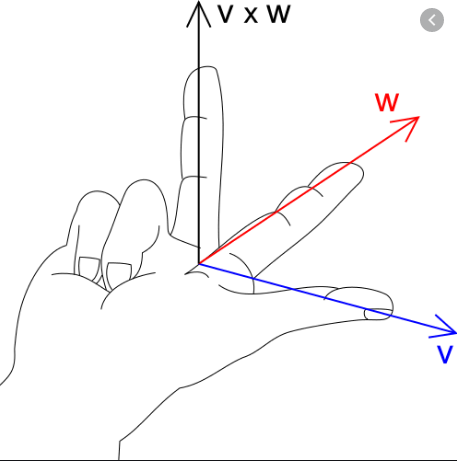
\includegraphics[width=2.6in]{regolaManoDestra.png}
  	\caption{Regola della mano destra per il calcolo del prodotto vettoriale}
   	\label{fig:manoDestra}
\end{figure}


%Di conseguenza, sui corpi che li contengono\footnote{C\'e una analogia con il campo elettrico: dato una carica elettrica, intorno ad essa si genera un campo elettrico $\vec{E}$, ossia l'induzione di una forza, attrattiva o repulsiva, su una seconda carica presente nelle vicinanze.}.



\'E per questo motivo che un magnete può generare forze su
\begin{itemize}
	\item un metallo, inducendo una corrente elettrica al suo interno
	\item un altro magnete che, per la definizione data, presenta delle correnti elettriche interne permanenti
\end{itemize}
	
	
	
	
	
	 

	
\begin{figure}[bh!]
	\centering
   	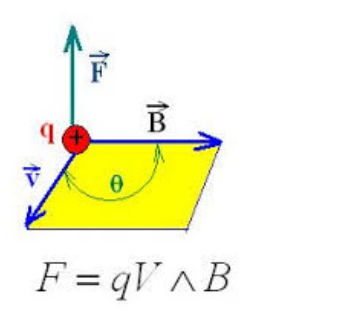
\includegraphics[width=2.6in]{ForzaLorentz.png}		%regolaManoDestra.png
  	\caption{Forza di Lorentz generato da un campo magnetico su una carica elettrica avente velocità v}
   	\label{fig:ForzaLorentz}%ForzaLorentz.png
\end{figure}	
	
	
\begin{figure}[th]		%EffettoHall.png
	\centering
   	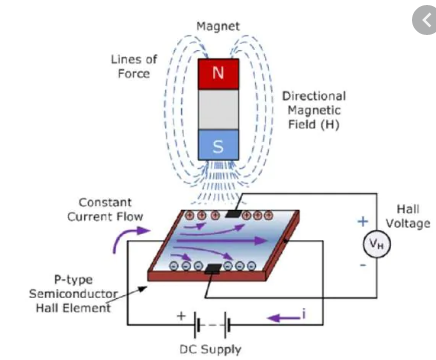
\includegraphics[width=3.0in]{EffettoHall.png}		%rettaNONpassOrig.jpg
  	\caption{Effetto Hall su un conduttore percorso da corrente dovuto alla Forza di Lorentz generata dal campo magnetico $\vec{B}$}
   	\label{fig:EffettoHall}%ForzaLorentz.png
\end{figure}	


	\item {\bf Legge di Faraday-Neumann: Tensione indotta}
	
	
	
	Se \'e presente un circuito elettrico chiuso \emph{concatenato} con il campo magnetico, allora si genera una forza elettromotrice indotta $E$ (si esprime in Volt)\footnote{Quando il circuito chiuso e la linea di campo magnetico costituiscono due linee di cui una passa dentro l'area chiusa dell'altra e viceversa, si dice che circuito e campo magnetico sono \emph{concatenati}.} che, matematicamente, \'e data dall'equazione
\begin{eqnarray}\label{eq:FaradayNeunman}
	E = -\frac{\Delta (SB_{\perp})}{\Delta t}
\end{eqnarray}	
	
	%$\frac{\Delta (SB)}{\Delta t} = - f.e.m.$, 
	ove $S$ rappresenta l'area chiusa dentro il circuito, $B$ è il modulo de campo magnetico e $B_{\perp}$ è quella componente di $B$ \emph{perpendicolare} al piano ove giace l'area $S$. $\phi(\vec{B}) = SB_{\perp}$ si chiama \emph{flusso} del campo magnetico  e si misura in \emph{Werber}\footnote{Il flusso del campo magnetico, pi\'u in generale, viene definito e calcolato per mezzo di integrali.}. %La Legge di Faraday-Neunmann \'e alla base del funzionamento dell'induttanza e del \emph{trasformatore}.





\subsection{Filo rettilineo percorso da corrente}

Per semplicità, proponiamo, come primo esempio, un filo rettilineo percorso da una corrente $i$, ad esempio $10$ $mA$ (figura \ref{fig:FiloRettilineoCorrente_B}). 
Intorno a tale filo si genera un campo magnetico $\vec{B}$. Come si può vedere dalla figura, in ogni punto la sua direzione \'e tangente alla linea di campo, quindi \emph{perpendicolare} alla corrente che lo induce. Le linee di campo sono circonferenze (quindi linee \emph{chiuse}) centrate intorno alla corrente stessa (figura \ref{fig:FiloRettilineoCorrente_B}).




Il modulo $B$ del vettore campo magnetico $\vec{B}$ \'e dato dall'equazione\footnote{Talvolta questa equazione \'e riportata come \emph{Equazione di Biot-Savart}. In realtà l'equazione di Biot-Savart presenta una formula pi\'u generale, che fa uso del calcolo integrale e che determina il campo magnetico generato da una corrente elettrica, qualsiasi sia il percorso che essa compie. }

\begin{eqnarray}\label{eq:B}
	B = \frac{\mu_0\mu_r i}{2\pi r}
\end{eqnarray}
ove

\begin{itemize}
	\item $\mu_0 = 4\pi\cdot 10^{-7}H/m$ si chiama costante diamagnetica del vuoto
	\item $\mu_r$ costante diamagnetica relativa, \'e pari ad $1$ nel vuoto e, in generale, assume valori diversi a seconda del mezzo in cui \'e immerso il sistema
	\item $r$ \'e la distanza del punto ove si calcola il campo magnetico con il filo
\end{itemize}



Nell'esempio precedente a distanza di $1$ $cm$ dal filo si ha un campo magnetico pari a 
\begin{eqnarray}
	B = \frac{4\pi\cdot 10^{-7}\cdot 10\cdot 10^{-3}}{2\pi \cdot 1\cdot 10^{-2}} = 2\cdot 10^{-7} \textrm{ Tesla}
\end{eqnarray}




%Pi\'u in generale, ogni volta che \'e presente una corrente, intorno ad essa si genera un campo magnetico $\vec{B}$ la cui natura matematica dipende, chiaramente, dalla geometria del percorso della corrente stessa e, di conseguenza, pu\'o presentare una notevole complessit\'a matematica. 

\subsection{Dipolo magnetico}




Come secondo esempio trattiamo il campo magnetico indotto da una corrente che scorre su una circonferenza chiusa. In tal caso si parla di \emph{dipolo magnetico}. In figura \ref{fig:dipoloMagnetico} è riportata una rappresentazione grafica delle linee di campo generate da un dipolo magnetico. \'E bene precisare che le linee di campo magnetico sono \emph{sempre} chiuse, soltanto che nel presente disegno alcune di esse si chiudono "molto lontano" dal dipolo.
Come sempre, le linee di campo rappresentano, punto per punto, la direzione del vettore campo magnetico $\vec{B}$. 

Il calcolo del campo indotto da un dipolo magnetico \'e assai complesso e qui viene omesso. Ci soffermiamo soltanto sul suo valore al centro della circonferenza. In tale punto il campo magnetico \'e diretto perpendicolarmente rispetto al piano della circonferenza e il suo modulo \'e espresso da una formula che, matematicamente, \'e identica all'equazione \ref{eq:B}, che qui riportiamo




















\begin{eqnarray}\label{eq:B1}
	B = \frac{\mu_0\mu_r i}{2\pi r}
\end{eqnarray}







In questo contesto con $r$ si intende il raggio della circonferenza ove passa la corrente.





\begin{figure}[bh!]
	\centering
   	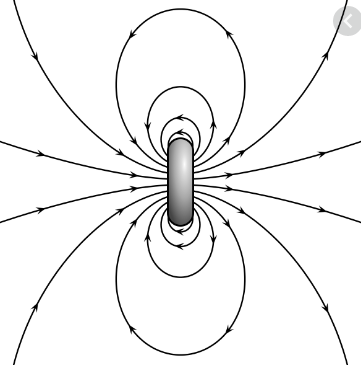
\includegraphics[width=2.3in]{dipoloMagnetico.png}%speakerMagneticField.gif
  	\caption{Linee di campo magnetico generate da un dipolo magnetico, la corrente scorre su una traiettoria circolare disposta perpendicolarmente al foglio.}
   	\label{fig:dipoloMagnetico}%bussola.png
\end{figure}



Un esempio di dipolo magnetico è l'ago della bussola che, sottoposta ad una coppia di forze dovute al campo magnetico terrestre, ruota fino a orientarsi in modo tale da \emph{annullare} la coppia di forze magnetiche su di essa agente

\begin{figure}[th!]
	\centering
   	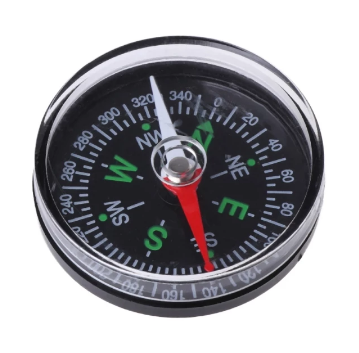
\includegraphics[width=2.4in]{bussola.png}%speakerMagneticField.gif
  	\caption{L'ago della bussola è costituito da un dipolo magnetico che ruota sotto l'effetto della coppia generata dal campo magnetico terrestre.}
   	\label{fig:bussola}%
\end{figure}


























\section{Basi di elettronica}
%\section{Generalità}

Per ragioni di completezza, passiamo in breve rassegna alcune delle grandezze e delle leggi fondamentali dell'elettronica:
la \emph{Prima Legge di Ohm} 

\begin{eqnarray}
	\Delta V = RI
\end{eqnarray}

ove  
\begin{itemize}
	\item $\Delta V$ è la tensione (Volt)
	\item $R$ la resistenza (Ohm) matematicamente è una quantità reale, quindi un elemento circuitale puramente resistivo non genera \emph{sfasamento} tra tensione e corrente
	\item \begin{eqnarray}\label{eq:current}
		I = \frac{Q}{\Delta t}
	\end{eqnarray} l'Intensità di corrente elettrica (Ampere) che, per definizione, è la carica $Q$ espressa in $Coulomb$ diviso l'unità di tempo espresso in secondi.
\end{itemize}


\subsection{Condensatore}
Un condensatore è costituito da due conduttori (armature) molto vicini tra loro che non si toccano, funge da accumulatore di carica elettrica, è caratterizzato dalla capacità

\begin{eqnarray}
	C = \frac{Q}{\Delta V} %= \epsilon\frac{S}{d
\end{eqnarray}


il simbolo circuitale è riportato in figura \ref{fig:condensatoreSimbolo} e il valore della capacità è legato alle caratteristiche fisiche del condensatore per mezzo dell'equazione  

\begin{eqnarray}
	C = \frac{S\epsilon}{d}
\end{eqnarray}

ove
\begin{itemize}
	\item $S$ è l'area delle armature
	\item $\epsilon = \epsilon_0 \epsilon_r$ è il prodotto della costante dielettrica del vuoto $\epsilon_0 = 8.9\cdot 10^{-12}C^2/(Nm^2)$ e la costante dielettrica relativa $\epsilon_r$ che dipende dal dielettrico presente tra le armature
	\item $d$ è la distanza tra le due armature 
\end{itemize}



%\begin{eqnarray}
%	f(x) = x -\frac{\log(x)}{1-\sin x}
%\end{eqnarray}



\begin{figure}[b!]		
	\centering
   	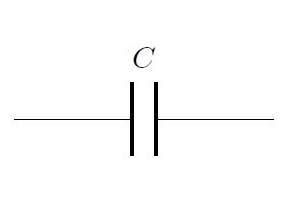
\includegraphics[width=1.8in]{condensatoreSimbolo.png}
  	\caption{Simbolo del condennsatore.}
   	\label{fig:condensatoreSimbolo}
\end{figure}


\begin{figure}[t]		
	\centering
   	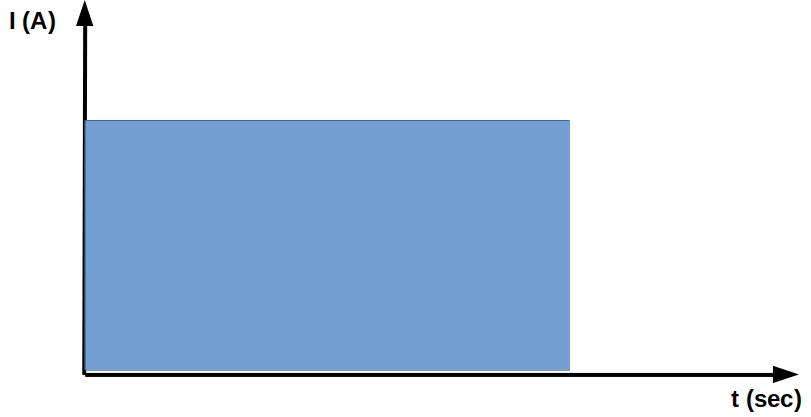
\includegraphics[width=2.5in]{correnteContinua_tempo_grafico.jpg}
  	\caption{Grafico della corrente continua in funzione del tempo. La carica è data dall'area del rettangolo $Q =It$.}
   	\label{fig:condensatoreSimbolo}
\end{figure}


Invertendo l'equazione \ref{eq:current}, si ottiene che la carica elettrica è il prodotto dell'intensità di corrente elettrica per il tempo $Q = It$. %Tuttavia questa espressione per la carica elettrica, che sarebbe valida in caso di corrente continua, è valida soltanto per intervalli di tempo molto ristretti poichè, come è ben noto, quando è presente un condensatore la corrente passa nel circuito soltanto per un breve intervallo di tempo necessario per caricare il condensatore stesso, dopodichè si estingue e il condensatore rimane sotto carica.



Su un grafico corrente - tempo (figura \ref{fig:condensatoreSimbolo}), la carica elettrica circolante in un tempo $t$ data dall'equazione $Q = it$ è l'area di quel rettangolo che sta tra la retta che rappresenta la corrente, l'asse delle ascisse, l'istante temporale iniziale ($t = 0$) e quello finale ($t$).







\begin{figure}[b!]		
	\centering
   	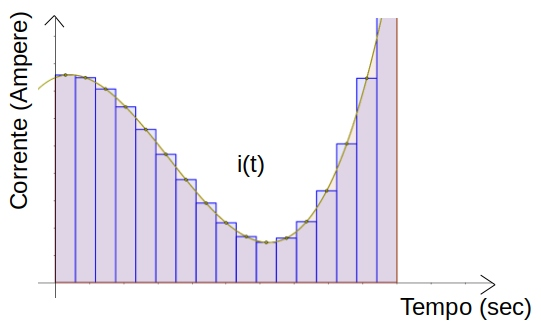
\includegraphics[width=2.5in]{integraleCorrente.jpg}
  	\caption{Grafico della corrente \emph{non} continua in funzione del tempo. La carica è data dall'area dell'area sotto la funzione e quindi l'integrale $Q =\int_{t_1}^{t_2}i(t)dt$.}
   	\label{fig:integraleCorrente}
\end{figure}%sfasamento

Quando la corrente \emph{non} \'e continua allora il suo andamento viene espresso per mezzo di una funzione matematica $y = f(x)$, ove $y$ è il valore della corrente e $x$ è il valore del tempo. La funzione matematica viene quindi rinominata $i = i(t)$ (linea continua figura \ref{fig:integraleCorrente}) e la carica accumulata è sempre l'area che sta tra la curva $i(t)$, l'asse delle ascisse e gli istanti temporali iniziale ($t_1$) e finale ($t_2$), soltanto che ora tale area si calcola con un integrale anzichè una semplice moltiplicazione base per altezza





\begin{eqnarray}
	Q = \int_{t_1}^{t_2}i(t)dt
\end{eqnarray}




Quindi la tensione di un condensatore è proporzionale all'integrale della corrente nel tempo

\begin{eqnarray}\label{eq:condensatoreIntegrale}
	E = \frac{1}{C}\int_{t_1}^{t_2}i(t)dt
\end{eqnarray}


Supponiamo che l'andamento della corrente elettrica nel tempo sia di tipo sinusoidale. 

\begin{eqnarray}
	i(t) =i_0\sin(\omega t)
\end{eqnarray}

Ove $i_0$ è l'ampiezza massima (ad esempio $2$ $A$) di corrente e $\omega$ è $2\pi$ moltiplicato per la frequenza $f$ (ad esempio $620$ $Hz$). Considerata l'equazione \ref{eq:condensatoreIntegrale}, per trovare la carica acumulata in un intervallo di tempo $t_2 - t_1$ occorre svolgere l'integrale

\begin{eqnarray}\label{eq:int1}
	E = \frac{1}{C} \int_{t_1}^{t_2}i(t)dt = \frac{1}{C}i_0\int_{t_1}^{t_2}\sin(\omega t)dt 
\end{eqnarray} 


La risoluzione dell'integrale di cui \ref{eq:int1}

\begin{eqnarray}\label{eq:ritFase}
	\Delta E = - \frac{1}{\omega C} i_0\cos(\omega t)
\end{eqnarray}

%Tra tensione e corrente c'\'e uno sfasamento che coincide con

Lo sfasamento tra tensione e corrente è quindi lo sfasamento che risulta tra $-\cos(\omega t)$ e $\sin(\omega t)$, riportato in figura \ref{fig:sfasamento}.  


\begin{figure}[b!]		
	\centering
   	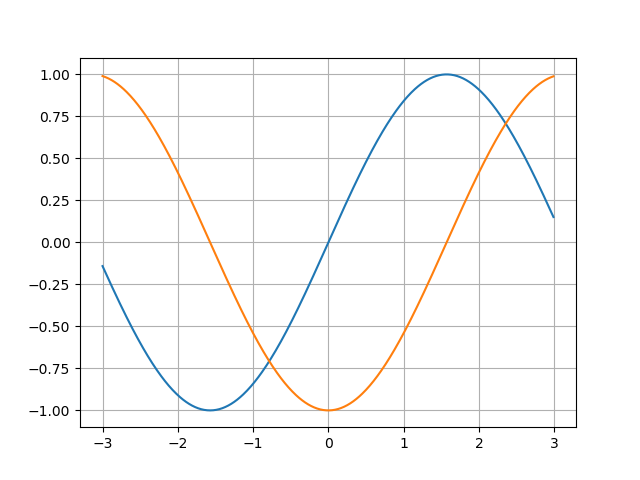
\includegraphics[width=3.5in]{sfasamento.png}
  	\caption{Linea blu \'e il grafico della funzione $\sin(x)$, la linea rossa \'e il grafico della funzione $-\cos(t)$.}
   	\label{fig:sfasamento}
\end{figure}%


La funzione $-\cos(t)$ (linea rossa) è in ritardo rispetto alla funzione $\sin(t)$ (linea blu) di $\pi/2 \approx 1.57$. Quindi in un condensatore si presenta uno \emph{sfasamento} tale per cui la tensione presenta un \emph{ritardo} rispetto alla corrente. 

Se si esclude per un momento il ritardo di fase, nella equazione \ref{eq:ritFase} l'impedenza è pari al rapporto tra tensione e corrente


\begin{eqnarray}
	Z = \frac{1}{\omega C}
\end{eqnarray}

L'unità immaginaria che solitamente si usa esprime, appunto, il fatto che tra tensione e frequenza \emph{non} c'è soltanto un fattore di proporzionalità, senza alcuno sfasamento, come accade per le resistenze, ma anche un ritardo di fase come appena descritto.


\begin{eqnarray}
	Z = \frac{1}{j\omega C}
\end{eqnarray}



\subsection{Induttore}

L'induttore è un elemento circuitale passivo costituito da un solenoide avvolto intorno ad un ferromagnete. Il simbolo è riportato nella figura \ref{fig:simboloInduttore}. 

Una corrente elettrica passante attraverso un solenoide, o induttore, (costituito da un filo che descrive una geometria ad elica) genera un campo magnetico $\vec{B}$ che si concatena con l'induttore stesso e che, all'interno di esso, ha direzione perpendicolare ai piani delle spire circolari del solenoide (figura \ref{fig:induttanza}). 

Si dimostra che l'intensità di questo campo magnetico è proporzionale alla corrente $i$ e il numero di avvolgimenti $N$\footnote{Secondo il Teorema della Circuitazione di Ampere, l'integrale $\oint_{\gamma}\vec{B}\cdot d\vec{s} = \mu_0\mu_r i$, applicato ad un circuito $\gamma$ che passa per l'asse centrale del solenoide e si estende all'infinito, si ha che l'integrale diventa il prodotto del campo magnetico (costante) $B$ moltiplicato per la lunghezza $l$ del solenoide, da cui si ricava l'equazione \ref{eq:Bsolenoide} }, secondo la formula



\begin{eqnarray}\label{eq:Bsolenoide}
	B = \frac{\mu_0\mu_r iN}{l}
\end{eqnarray}



%\vspace{3cm}



	
%Fsi\section{L'induttore}



%\begin{eqnarray}
%	B = \frac{\mu_0\mu_r iN}{l}
%\end{eqnarray}

ove
\begin{itemize}
	\item	$\mu_0$ \'e la costante diamagnetica
	\item	$i$ la corrente elettrica in Ampere
	\item	$N$ il numero di spire
	\item	$l$ la lunghezza dell'induttanza
\end{itemize}


\begin{figure}[bh!]
	\centering
   	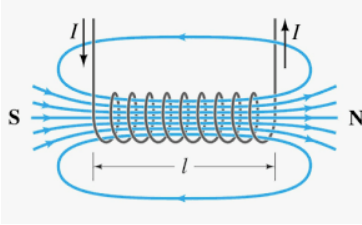
\includegraphics[width=3.5in]{Induttanza.png}%coppiaMotoreDC
  	\caption{Induttanza e linee di campo magnetico autoconcatenate.}
   	\label{fig:induttanza}
\end{figure}


Ciò che conta della precedente formula \'e che il campo magnetico autoconcatenato con la spira \'e \emph{proporzionale} alla corrente e si scrive
\begin{eqnarray}
	B \propto i
\end{eqnarray}

Come conseguenza, anche la variazione nel tempo del campo magnetico \'e proporzionale alla variazione nel tempo della corrente elettrica
\begin{eqnarray}
	\frac{\Delta B}{\Delta t} \propto \frac{\Delta i}{\Delta t}
\end{eqnarray}


Dalla Legge di Faraday-Neunman (equazione \ref{eq:FaradayNeunman}), a seconda della natura della corrente elettrica, si hanno due situazioni distinte:


\begin{enumerate}
	\item se è {\bf continua} allora la variazione nel tempo del flusso de campo magnetico concatenato con il circuito è nulla, \emph{non} si genera una tensione ai capi dell'elemento circuitale e l'induttanza è un {\bf cortocircuito}%\footnote{Mentre invece la capacitanza è un circuito aperto.}  

	\item Se è {\bf alternata}, invece, anche il campo magnetico $\vec{B}$ e il flusso $SB_{\perp}$ sono alternati e quindi si sviluppa una {\bf tensione} pari a%\footnote{Mentre invece la capacitanza va come l'integrale della corrente nel tempo.}
\end{enumerate}
\begin{figure}[b!]		
	\centering
   	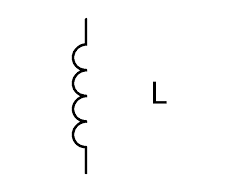
\includegraphics[width=1.5in]{induttoreSimbolo.png}%sfasamento1.png
  	\caption{Simbolo circuitale dell'induttore.}
   	\label{fig:simboloInduttore}
\end{figure}%



\begin{eqnarray}
	E = -\frac{\mu_0\mu_r SN^2}{l}\frac{\Delta i}{\Delta t} = L\frac{\Delta i}{\Delta t}
\end{eqnarray}

%Ove il coefficiente di proporzionalità tra la tensione e la derivata della corrente elettrica prende il nome di induttanza, l'unità di misura è l'Henry ed è
ove
\begin{eqnarray}
	L = -\frac{\mu_0\mu_r SN^2}{l}
\end{eqnarray}

\'E l'induttanza e si esprime in \emph{Henry} ($H$).

Condensatore e induttore hanno un comportamento opposto l'uno rispetto all'altro al passaggio della corrente: mentre la risposta in tensione del condensatore è proporzionale all'integrale nel tempo della corrente elettrica (con coefficiente di proporzionalità $1/C$), la risposta in tensione di un induttanza è proporzionale alla derivata della corrente elettrica nel tempo.


 


Come nel caso del condensatore, così anche in questo caso supponiamo che la corrente abbia un andamento sinusoidale nel tempo:

\begin{eqnarray}
	i(t) = i_0 \sin(\omega t)
\end{eqnarray}

Essendo la sua derivata pari a $i_0\omega \cos(\omega t)$, si ottiene una tensione pari a

\begin{eqnarray}
	E = \omega L i_0\cos(\omega t)
\end{eqnarray}

A meno di un fattore di fase, il coefficiente di proporzionalità, che chiamiamo impedenza, è 

\begin{eqnarray}
	Z = \omega L
\end{eqnarray}

L'unit\'a immaginaria che notoriamente si usa per caratterizzare l'impedenza di una induttanza

\begin{eqnarray}
	Z = j\omega L
\end{eqnarray}

 tiene conto della differenza di fase che è presente tra tensione e corrente. Quindi mentre nel condensatore la tensione è in anticipo rispetto alla corrente di un valore $\pi/2$, nell'induttanza la tensione è in \emph{ritardo} rispetto alla corrente dello stesso valore $\pi/2$.


\begin{figure}[b!]		
	\centering
   	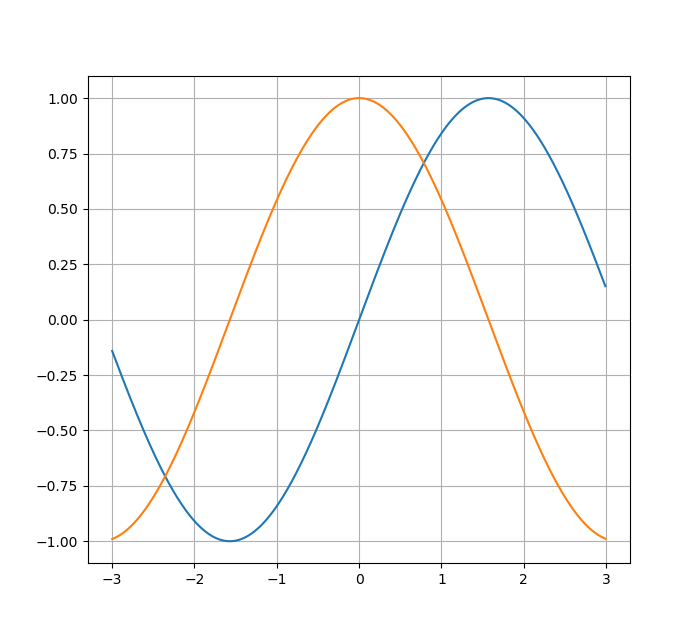
\includegraphics[width=3.2in]{sfasamento1.png}
  	\caption{Sfasamento tra la funzione $\sin(t)$ (corrente, linea blu), e la funzione $\cos(t)$ (tensione, linea rossa). Nell'induttanza la tensione è in anticipo rispetto alla corrente.}
   	\label{fig:sfasamento1}
\end{figure}%




\section{Trasformatore}

Il trasformatore \'e costituito da due solenoidi detti, rispettivamente, \emph{primario} e \emph{secondario}. Se sul primo solenoide si applica una corrente elettrica \emph{continua}, ossia non variabile nel tempo, intorno ad essa si genera un campo magnetico $\vec{B}$, anch'esso \emph{non} variabile nel tempo. Un tale campo magnetico non sarà mai in grado di generare una forza elettromotrice indotta su una seconda spira perch\'e, come descritto dalla legge di Faraday-Neumann (equazione \ref{eq:FaradayNeunman}), questa \'e pari alla variazione nel tempo del flusso del campo magnetico cambiata di segno.

Affinch\'e il solenoide primario generi una forza elettromotrice indotta sul solenoide secondario, \'e necessario che esso generi un campo magnetico \emph{variabile} nel tempo, ciò è possibile \emph{soltanto} se sul primario passa una corrente elettrica \emph{alternata}. 


%In pratica, la variazione nel tempo del campo magnetico generato dal solenoide primario e concatenato sul solenoide secondario sarà proporzionale alla variazione nel tempo della corrente elettrica applicata sul solenoide primario

%\begin{eqnarray}
%	\frac{\Delta i_{\textrm{primario} } }{\Delta t}\propto \frac{\Delta B_{\textrm{secondario}}}{\Delta t}
%\end{eqnarray}

Applicando una tensione alternata $V_1(t)$ sul circuito primario del trasformatore, si genera su di esso una corrente $i_1(t)$ e, di conseguenza, un campo magnetico $B_1(t)$ che supponiamo si concateni perfettamente con il circuito secondario l'equazione

\begin{eqnarray}
	B_2(t) = \frac{\mu_0\mu_r i_1(t)N_1}{l}\propto V_1(t)
\end{eqnarray}

A sua volte, il campo magnetico $B_2(t)$ sviluppa una tensione $V_2(t)$ sul circuito secondario costituito da $N_2$ spire.

Da questa osservazione si deduce (con dei passaggi matematici che, al momento, ometto) che la forza elettromotrice indotta sul solenoide secondario dovuto alla corrente elettrica alternata sul primario \'e data dalla formula

\begin{eqnarray}
	\frac{V_1}{V_2} = \frac{N_1}{N_2}
\end{eqnarray}

Ove




\begin{itemize}
	\item $V_1$ \'e la tensione applicata al solenoide primario
	\item $V_2$ \'e la tensione applicata al solenoide secondario
	\item $N_1$ \'e il numero di spire presenti sul solenoide primario
	\item $N_2$ \'e il numero di spire presenti sul solenoide secondario
\end{itemize}
\end{enumerate}
	


\section{Trasduttore acustico}\label{par:OndaMeccanica}


Il suono è una onda meccanica. Ossia una perturbazione locale dello stato di pressione (forza per unità di superficie) e densità (massa per unità di volume) dell'aria che si propaga nello spazio e nel tempo. La velocità di propazione del suono è, mediamente, $c_s = 340$ $m/s$ (circa $1200$ $km/h$) e può variare di qualche percentuale a seconda della consistenza del mezzo attraverso il quale passa (\emph{impedenza acustica}). Il suono è caratterizzato dalla frequenza ($\nu$) e lunghezza d'onda ($\lambda$)\footnote{Un altro tipo di onde sono le onde elettromagnetiche capitolo \ref{cap:elettromagnetiche}, che costituiscono una perturbazione nello spazio e nel tempo del campo elettromagnetico e viaggiano ad una velocità molto più alta (velocità della luce $c = 3\cdot 10^8m/s$)}, le quali sono legate tra di loro per mezzo della relazione
\begin{eqnarray}
	\lambda \nu = c_s
\end{eqnarray}




\begin{figure}[t]
	\centering
   	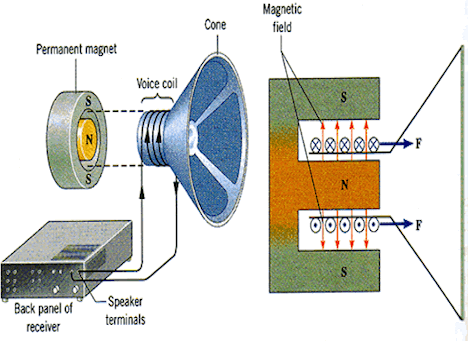
\includegraphics[width=4.4in]{speakerMagneticField.png}%speakerMagneticField.gif
  	\caption{Principio di funzionamento di un altoparlante (trasduttore acustico).}
   	\label{fig:trasduttoreSuono}
\end{figure}




L'orecchio umano è in grado di percepire intervalli di frequenza di segnali acustici che va da $20$ $Hz$ a $20$ $kHz$. Segnali acustici caratterizzati da frequenza \emph{superiore} a $20$ $kHz$ sono \emph{ultrasuoni}. Segnali acustici caratterizzati fa frequenze \emph{inferiori} a frequenze acustiche sono \emph{infrasuoni}. 


La propagazione di onde meccaniche non si manifesta soltanto in qualità di suono, ma si può manifestare, ad esempio, anche in qualità di trasmissione di energia sotto forma di calore.
Quando una particella, come ad esempio un elettrone, assorbe l'energia proveniente da un onda meccanica, si dice che tale particella \emph{assorbe un fonone}. Allo stesso modo, quando una particella assorbe energia proveniente da un onda elettromagnetica, si dice che tale particella \emph{assorbe un fotone}. 
Queste considerazioni risulteranno utili quando, nel paragrafo \ref{par:trasdSemicon}, si tratteranno i trasduttori di temperatura.



























Il microfono, evidentemente, è un trasduttori acustico, cioè un dispositivo in grado di trasdurre un segnale elettrico in acustico. L'altoparlante, invece, è un dispositivo che, sempre sulla base dello stesso principio di funzionamento, esegue la trasduzione opposta, cioè converte il segnale elettrico in acustico.

La figura \ref{fig:trasduttoreSuono} riporta uno schema di funzionamento di un altoparlante. Esso è costituito da uno statatore con una cavità dove è presente un campo magnetico $\vec{B}$ al suo interno, avente direzione radiale. Al passaggio di corrente attraverso la bobina contenuta nella cavità circolare dello statore, si genera una Forza di Lorentz (equazione \ref{eq:Lorentz}) che spinge la bobina, e quindi il cono di cartone ad essa vincolata, in direzione ortogonale alla corrente e al campo magnetico $\vec{B}$.

La spinta del cono di cartone genera la perturbazione di pressione e densità dell'aria che, come accennato a inizio paragrafo, costituisce l'essenza stessa del suono.
























\clearpage

\section{Motore in corrente continua}


In generale, il motore in corrente continua è composto da
\begin{itemize}
	\item statore
	\item rotore
	\item collettore con spazzole o commutatore
\end{itemize}

In figura \ref{fig:motoreCorrenteContinua} è riportata la configurazione più elementare possibile di un motore in corrente continua. Lo statore, costituito da due estensioni polari opposte (rispettivamente nord e sud magnetico), presenta una cavità all'interno del quale induce un campo magnetico $\vec{B}$ 

 \begin{figure}[bh!]		
	\centering
   	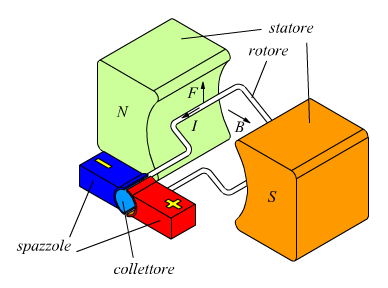
\includegraphics[width=4.8in]{motoreCorrenteContinua.png}
  	\caption{Schema del motore in corrente continua.}
   	\label{fig:motoreCorrenteContinua}
\end{figure}


Le estensioni polari possono essere costituite da
\begin{itemize}
	\item magneti permanenti 
	\item elettromagneti collegati in \emph{serie} con la bobina del rotore
	\item elettromagneti collegati in \emph{parallelo} con la bobina del rotore
\end{itemize} 
%Consideriamo, per semplicità, soltanto il primo caso.
Nella cavità dello statore è presente il rotore, ossia un corpo rigido (sezione \ref{cap:corpoRigido}) libero di muoversi intorno ad un asse di rotazione, avente un elettromagnete alimentato attraverso una coppia di contatti striscianti (spazzole) presenti sul \emph{collettore}.



%Il campo magnetico $\vec{B}$ nella cavità dello statore può essere generato da


Al passaggio di una corrente $i$ sulla bobina rotorica, rappresentata in figura da una linea chiusa rettangolare di colore bianco, secondo la Legge di Lorentz (equazione \ref{eq:Lorentz}), che riportiamo di seguito per comodità


\begin{eqnarray}\nonumber%\label{eq:Lorentz}
	\vec{F} = i\vec{l}\times\vec{B}
\end{eqnarray}

si genera su due dei quattro lati una forza perpendicolare sia alla direzione della corrente ($\vec{l}$) che al campo magnetico ($\vec{B}$). Dal momento che corrente $i$ e campo magnetico $\vec{B}$ sono perpendicolari tra loro lungo tutto il moto del rotore, {\bf l'intensità delle forze $\vec{F}$ data dall'equazione \ref{eq:Lorentz} è costante in modulo, direzione e verso durante tutto il moto del rotore} e vale

\begin{eqnarray}
	F = ilB
\end{eqnarray}

\begin{comment}
al passaggio della corrente elettrica $i$ nella bobina, e in particolare sui due lati $l$ perpendicolari alle linee di campo, secondo la Legge di Lorentz
\begin{eqnarray}
	\vec{F} = i\vec{l}\cdot \vec{B}
\end{eqnarray}
\end{comment}

Ciò che non è costante, durante il moto del rotore, è la distanza dei punti di applicazione delle due Forze di Lorentz. Infatti
{\bf la coppia di forze \emph{non} è sempre perpendicolare al braccio e quindi \emph{non} è costante durante il moto del rotore}

\begin{eqnarray}\label{eq:coppiaMotoreDC}
	M = ilbB\sin\alpha 
\end{eqnarray}

































































ove il prodotto  $lbB$ è il flusso $\phi$ generato dallo statore e $\sin(\alpha)$ è l'angolo che ciascuna delle due forze forma con il braccio $b$. L'equazione \ref{eq:coppiaMotoreDC} diventa

\begin{eqnarray}\label{eq:coppiaRotore}
	M = \phi(B)i\sin(\alpha)
\end{eqnarray}

Quindi, mentre la forza applicata sul rotore è costante lungo tutto il moto del rotore stesso, la coppia \emph{non} è costante e, anzi, è \emph{massima} quando la bobina è posizionata \emph{parallelamente} al campo magnetico $\vec{B}$ e \emph{minima} quando la bobina è disposta \emph{perpendicolarmente} rispetto alle linee di campo magnetico (figura \ref{fig:coppiaMotoreDC}). 



\begin{figure}[th!]
	\centering
   	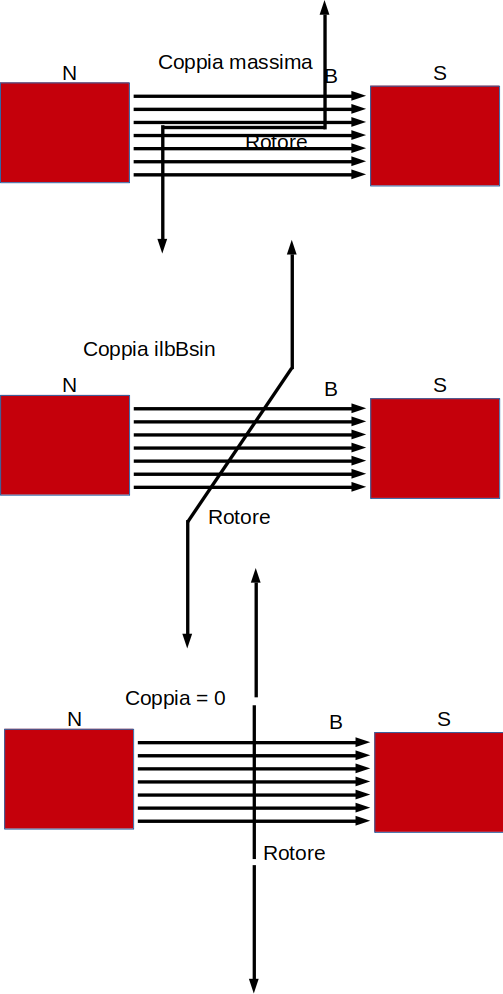
\includegraphics[width=2.6in]{coppiaMotoreDC.png}
  	\caption{Coppia applicata a un avvolgimento del rotore in funzione dell'angolo che esso forma con le linee di campo magnetico.}
   	\label{fig:coppiaMotoreDC}
\end{figure}



Evidentemente, per ottenere una coppia il più possibile costante lungo tutto il moto del rotore, una possibile soluzione è di disporre non un solenoide soltanto, ma più solenoidi, e/o più espansioni polari disposti con angolazioni diverse in modo tale che ad ogni angolo agisca non una sola coppia di Forze di Lorentz, ma più coppie con fasi differenti.

\subsection{Motore in corrente continua a eccitazioni indipendenti}

%\subsection{Controllo della coppia}

Dall'equazione \ref{eq:coppiaRotore} si evince che la coppia sul rotore è proporzionale alla corrente che lo attraversa. Si deduce quindi che, il controllo della coppia generata da un motore elettrico è possibile per mezzo del controllo della corrente su rotore.


La presente è la trascrizione della lezione disponibile sul sito

https://www.youtube.com/watch?v=5u-sSt55PMs

In figura \ref{fig:motoreDC_eccitazio indipendenti} è riportato il circuito di un motore in corrente continua a eccitazioni indipendenti. 


\begin{figure}[th!]
	\centering
   	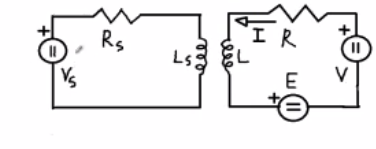
\includegraphics[width=3.3in]{motoreDC_eccitazioIndipendenti.png}
  	\caption{Coppia applicata a un avvolgimento del rotore in funzione dell'angolo che esso forma con le linee di campo magnetico.}
   	\label{fig:motoreDC_eccitazio indipendenti}
\end{figure}


\begin{itemize}
	\item $V_s$ è la tensione con la quale deve essere alimentato lo statore affichè esso possa generare un campo magnetico
	\item $R_s$ è la resistenza elettrica del filo conduttore costituente lo statore
	\item $L_s$ è l'induttanza del filo conduttore statorico
	\item $L$ è l'induttanza del filo conduttore rotorico
	\item $R$ è la resistenza elettrica del filo conduttore costituente il rotore
	\item $V$ è la tensione di alimentazione del rotore
	\item $E$ è detta forza controelettromotrice e si genera nel momento in cui il rotore entra in rotazione
\end{itemize}

La tensione $E$ è direttamente proporzionale alla velocità di rotazione angolare $\omega$ del motore

\begin{eqnarray}\label{eq:controEM}
	E = k_E\omega
\end{eqnarray}

Nel circuito di destra, applicando il Secondo Principio di Kirkhhoff si ha 
\begin{eqnarray}
	V = Ri + E
\end{eqnarray}

Ma sappiamo che la forza controelettromotrice è uguale a $k_E\omega$, pertanto l'equazione diventa la seguente

\begin{eqnarray}
	V = Ri + k_E\omega
\end{eqnarray}

Da cui si ricava l'espressione matematica della corrente assorbita dal motore

\begin{eqnarray}
	I = \frac{V-k_E\omega}{R}
\end{eqnarray}

La coppia motrice necessaria per far ruotare l'albero motore è direttamente proporzionale alla corrente sul rotore

\begin{eqnarray}
	C_m = k_Ti
\end{eqnarray}


Si definisce corrente di spunto la corrente assorbita dal motore nel momento in cui inizia a ruotare. In quell'istante il motore è fermo, quindi la corrente di spunto è

\begin{eqnarray}
	I_s = \frac{V}{R}
\end{eqnarray}

Che è evidentemente la massima corrente assorbita dal motore.

L'espressione matematica della coppia motrice $C_m$, essendo proporzionale alla corrente rotorica 

\begin{eqnarray}\label{eq:coppiaVelocit}
	C_m = k_Ti = k_T\left( \frac{V-k_E\omega}{R} \right) & = & k_TI_s- \frac{k_Tk_E}{R}\omega  \\ \nonumber
	y & = & q +  mx 
\end{eqnarray}

l'equazione \ref{eq:coppiaVelocit}, riportata su un opportuno grafico coppia-velocità angolare, da luogo a una retta con coefficiente angolare negativo ($k_Tk_E/R$) e intercetta pari a $k_TI_s$.


Quando $k_E\omega = V$ la corrente assorbita dal motore è nulla. Si dice che il motore è a \emph{regime}. In corrispondenza di tale configurazione la coppia motrice è nulla. \'E evidente che una tale configurazione è soltato ideale, perchè in un qualsiasi motore elettrico è sempre presente un attrito che limita la rotazione del rotore e che quindi rende necessario un passaggio di corrente e una coppia motrice, seppur minimi.



\clearpage

\section{Lo spettro elettromagnetico}\label{cap:elettromagnetiche}

Una onda elettromagnetica è una perturbazione del campo elettromagnetico che si propaga nello spazio e nel tempo. La propagazione avviene per mezzo di quanti di luce detti \emph{fotoni}. La velocità con cui si propaga un onda elettromagnetica è un valore costante\footnote{In realtà ci possono essere delle piccole variazioni percentuali indotte dal mezzo attraverso il quale l'onda si propaga. A tal proposito, si definisce \emph{indice di rifrazione} n di un materiale il coefficiente attraverso il quale si ricava la velocità $v$ dell'onda che lo attraversa, secondo la formula $v=c/n$. L'indice di rifrazione, inoltre, è spesso dipendente dalla lunghezza d'onda $\lambda$ della radiazione incidente. Questa non costanza della velocità della luce attraverso diversi mezzi è responsabile di fenomeni ottici quali, ad esempio, la distorsione di immagini viste attraverso l'acqua.} noto come velocità della luce. Un onda elettromagnetica viene emessa da un \emph{dipolo oscillante}, ossia una coppia di cariche elettriche, una positiva e una negativa, che si muovono intorno ad un centro di oscillazione. 

Tale perturbazione viene caratterizzata con

\begin{itemize}
	\item frequenza $\nu = \frac{1}{T}$ (inverso del periodo di oscillazione)
	\item lunghezza d'onda $\lambda$
	\item energia $\epsilon$\footnote{l'energia viene normalmente espressa in Joule per sistemi \emph{macroscopici} e in electronVolt ($1eV = 1.6\cdot 10^{-19}J$) per sistemi \emph{microscopici}.} di ogni singolo fotone
	\item Intensità $I$ (Vettore di Poynting) pari alla potenza $P$ per unità di superficie $I = \frac{P}{S}$
\end{itemize}

le prime tre di queste variabili sono legate tra loro per mezzo di due leggi fisiche

\begin{itemize}
	\item $\lambda\nu = c$
	\item $\epsilon = h\nu$ (Legge di Planck)
\end{itemize}

Ove la velocità della luce $c$ e la costante di Planck h valgono, rispettivamente
\begin{eqnarray}
	c & = & 3\cdot 10^8m/s\\
	h & = & 6.64\cdot 10^{-34}J\cdot s = 6.5\cdot 10^{-16} eV\cdot s
\end{eqnarray}


Come si vede nella figura \ref{fig:spettroElettromagnetico}, a seconda della frequenza o della lunghezza d'onda, le onde elettromagnetiche si dividono, principalemente in 

\begin{itemize}
	\item Onde radio
	\item Microonde
	\item Infrarossi
	\item visibile
	\item ultravioletto
	\item Raggi X
	\item Raggi $\gamma$
\end{itemize}

\begin{figure}[b!]		%bandeSemiconduttore
	\centering
   	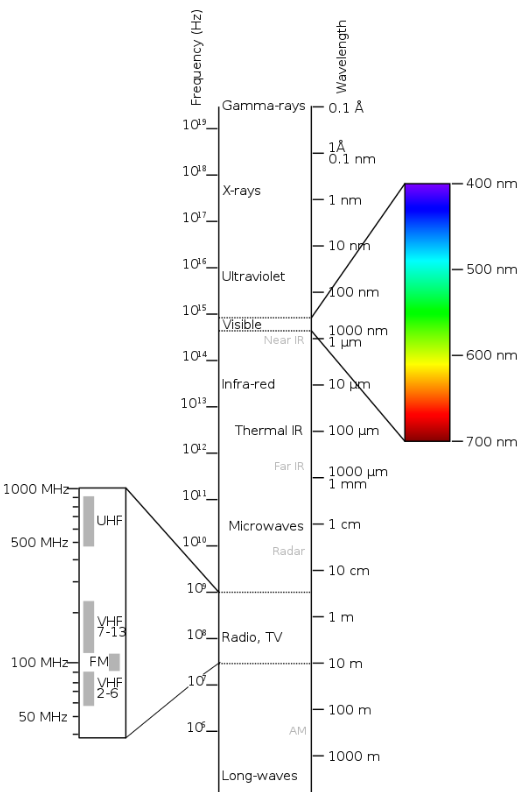
\includegraphics[width=3.3in]{spettroElettromagnetico.png}%PLC6ingressi6uscite.png
  	\caption{Spettro Elettromagnetico.}
   	\label{fig:spettroElettromagnetico}%ForzaLorentz.png
\end{figure}

In figura \ref{fig:spettroElettromagnetico}, si osserva che la luce visibile è quell'onda elettromagnetica dotata di una lunghezza d'onda compresa tra $400$ $nm$ e $700$ $nm$. Inoltre, all'interno dello spettro visibile, diversi colori corrispondono a diverse lunghezze d'onda. Ad esempio, il colore giallo corrisponde ad una lunghezza d'onda di circa $600$ $nm$, mentre il colore verde corrisponde a una lunghezza d'onda di circa $550$ $nm$. 

Sempre in figura \ref{fig:spettroElettromagnetico}, si osserva che l'\emph{ultravioletto} è quella onda elettromagnetica dotata di \emph{frequenza} $\nu$ \emph{superiore} alla frequenza del visibile, mentre l'\emph{infrarosso} è costituito da onde elettromagnetiche con \emph{frequenze} \emph{inferiori} rispetto al visibile. 

Infine, considerato il fatto che la lunghezza d'onda $\lambda$ è l'inverso della frequenza $\nu$, un discorso analogo su infrarosso e ultravioletto lo si può sulla base della lunghezza d'onda piuttosto che sulla base della frequenza: l'infrarosso è dotato di una lunghezza d'onda superiore rispetto al visibile, mentre l'ultravioletto è dotato di una lunghezza d'onda inferiore rispetto al visibile.


\subsection{Trasduttori a semiconduttore}\label{par:trasdSemicon}

Le proprietà elettriche dei semiconduttori dipendono principalmente dalla {\bf mobilità} e {\bf energia} degli elettroni in essi contenuti\footnote{Dipendono anche dal grado di cristallinità del materiale stesso, che non è una proprietà degli elettroni.}

\begin{itemize}
	\item {\bf Mobilità.} La possibilità che hanno gli elettroni di muoversi quando il materiale è sottoposto a una tensione. Evidentemente maggiore è il numero di elettroni che possono muoversi e maggiore è la conduttività del materiale.
	\item {\bf Energia.} L'energia che ciascun elettrone può possedere all'interno del materiale stesso. In linea di massima maggiore è l'energia di ciascun elettrone e maggiore è la conduttività del materiale. 	
\end{itemize}


	L'energia di ciascun elettrone, evidentemente molto piccola rispetto ai valori macroscopici ai quali siamo abituati, si esprime per mezzo di una unità di misura nota come \emph{elettronvolt} ($eV$). L'elettronvolt è pari al Joule ($J$) moltipicato per un numero molto piccolo che è la carica dell'elettrone $1.6\cdot 10^{-19}C$\footnote{L'elettronvolt è definito come l'energia acquistata da un elettrone quando è accelerato dalla differenza di potenziale di un volt.}

\begin{eqnarray}
	1 eV = 1J\cdot 1.69\cdot 10^{-19}
\end{eqnarray}

Ciascun elettrone può acquisire energia per mezzo di due processi distinti: 
\begin{itemize}
	\item l'assorbimento di energia da un onda elettromagnetica (vedi paragrafo \ref{cap:elettromagnetiche}, assorbimento di un fotone)
	\item l'assorbimento di energia da un onda meccanica (vedi paragrafo \ref{par:OndaMeccanica}, assorbimento di un fonone)
\end{itemize}
 
E' evidente, quindi, che i semiconduttori possono essere usati sia come trasduttori di temperatura che trasduttori di luce.
Tuttavia la trattazione, a livello fisico, non è così semplice. 

%Ad esempio, un onda elettromagnatica caratterizzata da una di lunghezza d'onda $\lambda = 400 nm$ (luce visibile viola) non può essere trasdotta da qualsiasi semiconduttore ma, come vedremo, diversi semiconduttori sono in grado di trsdurre al meglio diverse lunghezze d'onda

Gli elettroni nei semiconduttori, infatti, possono essere dotati di certi valori di energia e \emph{non} possono essere dotati di altri valori. Si parla, quindi, nel contesto delle energie degli elettroni, del concetto di \emph{bande di energia} permesse e \emph{bande di energia} proibite\footnote{In chimica ciascun elemento della tavola periodica differisce dagli altri per il fatto che i suoi elettroni possono avere \emph{soltanto} livelli di energia discreti (vedi spettro atomo di idrogeno). I materiali macroscopici, che non sono altro che agglomerati di atomi, si distinguono da atomi singoli, per il fatto che le energie permesse \emph{non} sono su livelli discreti, ma su b\emph{bande continue}. }.


\begin{itemize}
	\item Una {\bf banda di energia permessa} è costituita da valori di energia, espressi in $eV$, che gli elettroni possono avere.
	\item Una {\bf banda di energia proibita} è costitutita da valori di energia, sempre espressi in $eV$, che gli elettroni \emph{non} possono avere.
\end{itemize}

Normalmente, le bande di energia permessa sono due, la più bassa si chiama {\bf banda di valenza}, la più alta si chiama {\bf banda di conduzione} e sono separate tra loro da una banda di energia proibita caratteristica del semiconduttore usato (figura \ref{fig:bandeSemiconduttore}).

Se la temperatura è sufficientemente bassa e se non c'è assorbimento di luce, allora gli elettroni tendono a stare tutti in banda di valenza. Tuttavia la banda di valenza differisce da quella di conduzione, oltre che per i livelli energetici più bassi, anche per il fatto che gli elettroni in questa banda \emph{non} sono mobili. Gli elettroni in banda di valenza \emph{non} contribuiscono alla conduzione. Se però degli elettroni in banda di valenza assorbono energia\footnote{Nei semiconduttori ordinari (Silicio, GaAs, Germanio), a temperature ordinarie (300 K) si ha una piccola percentuale di elettroni in banda di conduzione e il semiconduttore \emph{non} si comporta da isolante. } e passano in banda di conduzione, allora diventano cariche mobili. Non solo! L'assenza di un elettrone in banda di valenza genera un ulteriore carica mobile, di segno positivo, che è la lacuna. 
Quindi, a causa della presenza di questi due tipi di cariche mobili (elettroni di conduzione e lacune di valenza) il materiale diventa quindi conduttivo.
%La caratteristica dei semiconduttori è che a temperature ordinarie (300 K) gli elettroni si trovano quasi tutti in banda di valenza. Tuttavia, quando una piccola percentuale di essi acquisisce una energia superiore alla banda proibita, saltano in banda di conduzione, diventano quindi portatori di carica negativa. Il salto di un elettrone da banda di valenza a banda di conduzione lascia, in banda di valenza, una lacuna, ossia l'assenza di un elettrone, che costituisce essa stessa una carica mobile, di segno opposto, quindi positivo.
%Soltanto gli elettroni in banda di conduzione possono muoversi.

%Quando si applica una tensione, gli elettroni in banda di valenza \emph{non} si muovono, non contribuiscono quindi alla corrente. Viceversa, gli elettroni in banda di conduzione si muovono e sono responsabili del passaggio di corrente

%Allo stesso modo, quando in banda di valenza viene a mancare un elettrone, si ha una \emph{lacuna}, ossia una carica elettrica positiva che può muoversi quando viene applicata una tensione.

\begin{table}[t]
\centering
\begin{tabular}{|l|c|}
\hline
Semiconduttore & banda proibita ($eV$) \\
\hline
Silicio & 1.7\\
GaAs & 1.4\\
Germanio & 0.67\\
\hline
\end{tabular}
\caption{Bande proibite di diversi semiconduttori}
\label{tab:template}
\end{table}







\begin{figure}[b!]		
	\centering
   	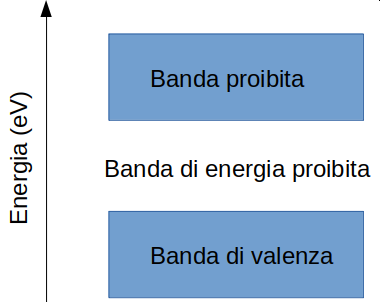
\includegraphics[width=2.3in]{bandeSemiconduttore.png}%PLC6ingressi6uscite.png
  	\caption{Bande di energia permesse (blu) e banda di energia proibita degli elettroni in un semiconduttore.}
   	\label{fig:bandeSemiconduttore}
\end{figure}



I semiconduttori, quindi, possono aumentare la loro conduttività aumentando la temperatura, possono quindi essere usati come {\bf termoresistenze}. Possono, inoltre, aumentare la loro conduttività aumentando l'esposizione alla luce, possono quindi essere usati come {\bf fotoresistenze}. 



\section{Cella fotovoltaica e fotodiodo}

%\vspace{2cm}
Oltre la termoresistenza, al fine di trasdurre la luce (dispositivo opto-elettronico) può essere usata la giunzione pn al Silicio. Più in generale, la giustapposizione di due materiali, non necessariamente a base di silicio, aventi proprietà elettroniche differenti, al quale si aggiunge l'uso di almeno uno dei due contatti elettrici trasparente alla luce, può convertire un segnale ottico che raggiunge la giunzione in un segnale elettronico.



I processi che sono alla base del funzionamento della giunzione pn, e quindi del trasduttore optoelettronico sono

\begin{itemize}
	\item diffusione di portatori di carica maggioritari attraverso la giunzione (cariche positive migrano verso la zona "n", cariche negative migrano verso la zona "p").
	\item eliminazione di portatori di carica liberi in una ristretta regione (regione di svuotamento) in corrispondenza della giunzione
	\item generazione di una differenza di potenziale a destra e a sinistra della giunzione, che favorisce il passaggio di carica elettrica in una direzione e lo ostacola nell'altra (diodo)
\end{itemize}

Al momento in cui un fotone raggiunge la regione di svuotamento della giunzione, può essere assorbito da un elettrone e genera una coppia elettrone-lacuna, responsabile di un passaggio di corrente in un eventuale circuito esterno al dispositivo stesso.



Il principale parametro usato per caratterizzare la cella fotovoltaica è il rendimento $\eta$ che esprime la percentuale di potenza luminosa convertita in potenza elettrica

\begin{eqnarray}\label{eq:efficienza}
	\eta = \frac{P_{el}}{P_{luce}} = \frac{VJ}{P_{luce}}
\end{eqnarray}

Valori tipici di efficienza di dispositivi fotovoltaici oscillano da qualche unità percentuale ($1\%$ o $2\%$ per dispositivi sperimentali) fino a oltre il $20\%$ per dispositivi ad alta efficienza. 

La potenza elettrica generata dipende, oltre che dalla quantità di luce che investe il dispositivo, anche dal carico applicato ai capi del dispositivo stesso. Come si vedrà a seguire, a valori differenti della resistenza su carico corrispondono valori differenti sia della corrente $J$ che della tensione $V$.

\vspace{1cm}

Da un punto di vista elettrico, la cella fotovoltaica è un diodo e, al buio, la sua risposta elettrica è esattamente quella del diodo (figura \ref{fig:ivCharacteristicSolarCellDark}): la corrente passa soltanto in polarizzazione diretta mentre il dispositivo è interdetto in polarizzazione inversa. 


Anche la forma analitica della caratteristica corrente tensione del dispositivo fotovoltaico al buio è identica a quella del diodo

\begin{eqnarray}\label{eq:ivBuio}
	J = J_s\left(e^{qV/(nK_BT)}-1\right)
\end{eqnarray}

\begin{figure}[t!]		
	\centering
   	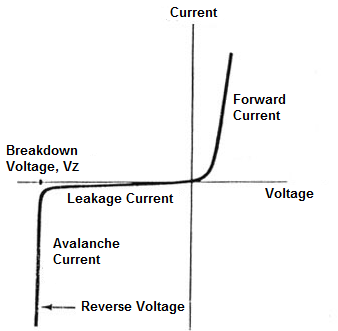
\includegraphics[width=3.3in]{ivCharacteristicsSolarCellDark.png}
  	\caption{Caratteristica IV di una cella solare \emph{al buio} }
   	\label{fig:ivCharacteristicSolarCellDark}
\end{figure}



ove
\begin{itemize}
	\item $J_s$ è la corrente di saturazione
	\item $q = 1.6\cdot 10^{-19}C$ è la carica dell'elettrone
	\item $K_B = 1.38\cdot 10^{-23}$ $JK^{-1}$ è la Costante di Boltzmann
	\item $n$ dipende dal semiconduttore utilizzato
	\item $T$ è la temperatura espressa in Kelvin
\end{itemize}

\vspace{2cm}

In figura \ref{fig:ivCharacteristicSolarCell}, invece, è riportata la caratteristica corrente tensione di un dispositivo fotovoltaico \emph{sotto illuminazione}. L'effetto fotovoltaico risulta, nella caratteristica IV, nella \emph{traslazione} della curva verso valori negativi della corrente.



Quindi, la forma analitica della caratteristica corrente tensione del dispositivo fotovoltaico sotto illuminazione, in prima approssimazione, è


\begin{eqnarray}
	J = J_s\left(e^{qV/(nK_BT)}-1\right) - J_{sc}
\end{eqnarray}

\begin{figure}[t]		
	\centering
   	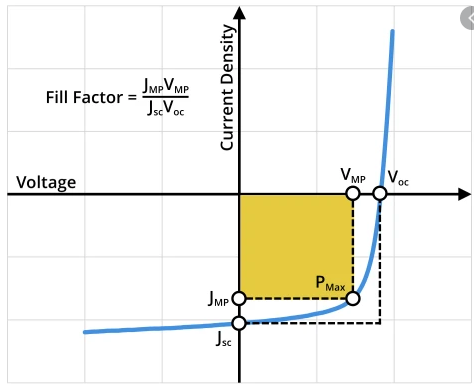
\includegraphics[width=3.3in]{ivCharacteristicsSolarCell.png}%ivCharacteristicsSolarCellDark
  	\caption{Caratteristica IV di una cella solare \emph{sotto illuminazione} }
   	\label{fig:ivCharacteristicSolarCell}
\end{figure}

ossia la caratteristica IV al buio (equazione \ref{eq:ivBuio}) \emph{meno} il valore della cosiddetta corrente di circuito aperto $J_{sc}$.




%E' chiaro che affinchè il dispositivo eroghi energia è necessario che sia sottoposto ad un carico. A parità di luce assorbita, differenti valori del carico corrispondono differenti valori della potenza elettrica generata. 
L'effetto fotovoltaico si ha soltanto quando al dispositivo è applicata una tensione tale per cui valori di tensione e corrente sono nel \emph{quarto quadrante} della figura \ref{fig:ivCharacteristicSolarCell}.


Da un punto di vista grafico, dato una coppia di valori $J$ e $V$, la potenza elettrica generata corrisponde all'area del rettangolo, disposto sul quarto quadrante della figura \ref{fig:ivCharacteristicSolarCell} di cui due dei quattro lati corrispondono alle coordinate del punto sulla curva.

%Ad un dato valore del carico applicato ad un dispositivo fotovoltaico associamo una differente retta di carico e quindi un differente punto sulla curva di figura \ref{fig:ivCharacteristicSolarCell}. 
%Per ciascuno di questi valori, la potenza elettrica sarà data dal prodotto di tensione $V$ per corrente $J$ e quindi dall'area del rettangolo formato dalle coordinate del punto sulla curva e gli assi coordinati.

%E' evidente che, a fini energetici, sarà importante trovare la retta di carico tale per cui l'area del suddetto rettangolo sia massimizzata. La coppia di valori di corrente e tensione che \emph{massimizza} l'area del



I principali parametri che si usano per caratterizzare un dispositivo fotovoltaico sono

\begin{itemize}%retta di carico
	\item Corrente di cortocircuito (\emph{S}hort \emph{C}ircuit Current $J_{sc}$)
	\item Tensione di circuito aperto (\emph{O}pen \emph{C}ircuit Voltage $V_{oc}$)
	\item Corrente di potenza elettrica massima $I_{MP}$
	\item Tensione di potenza elettrica massima $V_{MP}$
	\item Fattore di riempimento (Fill Factor $FF$) pari al rapporto tra l'area del rettangolo di potenza massima ($V_{MP}J_{MP}$)e l'area del rettangolo $J_{sc}V_{oc}$  ($FF =\frac{J_{sc}V_{oc}}{I_{MP}V_{MP}}$)
\end{itemize}

L'equazione dell'efficienza (equazione \ref{eq:efficienza}), quindi, può essere scritta anche così

\begin{eqnarray}
	\eta = FF\frac{J_{SC}V_{OC}}{P_{luce}}
\end{eqnarray}


%\vspace{2cm}

Il fotodiodo, invece, è un dispositivo fotovoltaico con un funziomento inverso rispetto alla cella fotovoltaica: quando viene attraversato da una corrente $J$ esso genera una potenza luminosa $P_{luce}$ la cui lunghezza d'onda (colore) dipende dalla band gap del semiconduttore utilizzato. Da un punto di vista elettrico, questo dispositivo, perchè si illumini, è un diodo che va collegato in \emph{polarizzazione inversa}. Da un punto di vista grafico, la regione di funzionamento del fotodiodo quando genera luce è disposta nel \emph{terzo quadrante} della figura \ref{fig:ivCharacteristicSolarCell}.




\clearpage

\section{PLC con sei ingressi e sei uscite}

In figura \ref{fig:PLC6ingressi6uscite} c'è un prototipo di PLC a sei ingressi che comanda sei motori in corrente continua a 24 Volt. 

Le uscite del PLC sono disposte alla destra della figura \ref{fig:PLC6ingressi6uscite} (da J12 a J17), ciascuna di esse è pensata per alimentare un motore elettrico in corrente continua per mezzo della tensione di alimentazione $V_{cc}$ da $24$ $Volt$. 



\begin{figure}[b!]		
	\centering
   	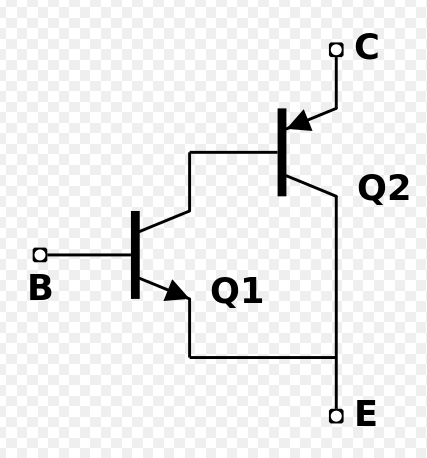
\includegraphics[width=2.3in]{coppiaDarlington.png}
  	\caption{Coppia Darlington}
   	\label{fig:coppiaDarlington}
\end{figure}

Il motore elettrico è un circuito di tipo \emph{induttivo}, capace quindi di generare delle \emph{tensioni di ritorno} quando il motore è in rotazione, come conseguenza della rotazione del circuito rotorico nel campo magnetico statorico (Legge di Faraday-Neumann-Lenz). Al fine di abbattere queste tensioni, ciascuna uscita del PLC presenta un \emph{diodo di ricircolo} (D1, D2, D3, D4, D5, D6, figura \ref{fig:motoreDC_diodoSoppressore}), capace di abbattere tensioni di ritorno in polarizzazione inversa. Le sei uscite sono comandate dai sei ingressi disposti nel basso della figura (J3, J4, J5, J7 J8 e J9). 

\begin{figure}[b!]		
	\centering
   	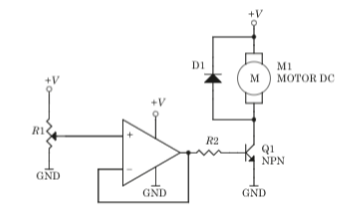
\includegraphics[width=3.3in]{motoreDC_diodoSoppressore.png}%ivCharacteristicsSolarCell.png
  	\caption{Alimentazione di un motore in corrente continua con commutatore BJT, buffer di tipo amplificatore operazionale, e diodo di soppressione (detto anche di \emph{ricircolo}) }
   	\label{fig:motoreDC_diodoSoppressore}
\end{figure}

Il reset del microcontrollore è stato usato anch'esso come ingresso. Di conseguenza, il reset viene effettuato spegnendo il microcontrollore. Tale operazione viene svolta in uscita dal LM7805, che controlla il commutatore costituito dalla coppia di BJT PNP disposti in basso a destra.




Come esempio di comando, al momento in cui al J4 viene applicato un segnale d'ingresso, il corrispettivo fototransistor viene portato in commutazione, collegando a ground ($0$ $Volt$) l'ingresso logico RB4 che a sua volta attiverà la relativa uscita dal PIC16F88, interfacciata con l'integrato ULN2003A.



L'ULN2003 è un integrato costituito da sei \emph{coppie Darlington} (figura \ref{fig:coppiaDarlington}), ossia sei amplificatori ciascuno avente come base l'uscita logica del microcontrollore. %La scelta della coppia Darlington è dovuta alla sua capacità di effettuare alte amplificazioni in corrente.



\begin{figure}[b!]		
	\centering
   	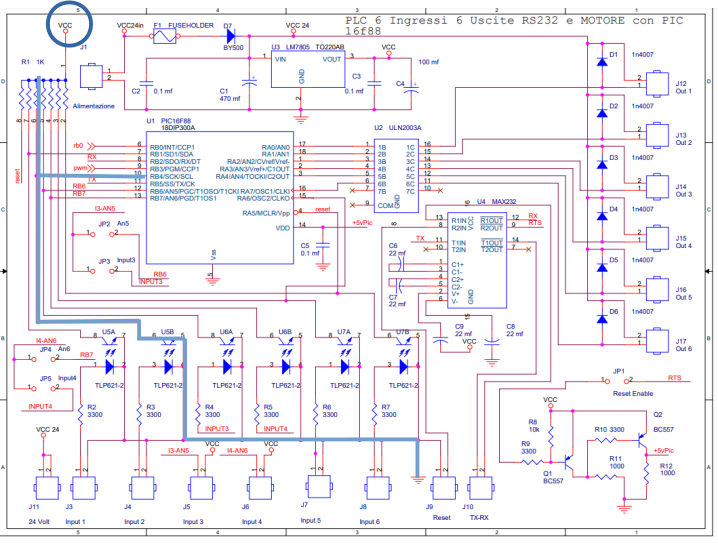
\includegraphics[width=5.8in]{PLC6ingressi6uscite.png}%coppiaDarlington.png
  	\caption{Progetto PLC con sei ingressi e sei uscite.}
   	\label{fig:PLC6ingressi6uscite}
\end{figure}




\end{document}